\documentclass[a4paper]{article}
\usepackage[pdftex]{graphicx}
\usepackage{anysize}
\marginsize{3cm}{3cm}{3cm}{3cm}
\usepackage[utf8]{inputenc}
\usepackage[T1]{fontenc}
\usepackage{enumitem}
\usepackage{titleref}

\usepackage[swedish]{babel}      
\usepackage{epstopdf}     % För svensk avstavning och svenska
\usepackage[osf]{mathpazo} % Palatino with smallcaps and oldstyle numbers
\usepackage[scaled]{helvet} % Helvetica, scaled 95%
\usepackage[titletoc]{appendix}

\usepackage{fancyhdr}

\fancyhf{}
\fancyhead[L]{Ansvarig: TG}
\fancyhead[R]{Datum: \today |Version: 0.7 | Dokumentnummer: PUSS144403}

\newcommand\invisiblesubsubsection[1]{%
  \refstepcounter{subsubsection}%
  \addcontentsline{toc}{subsubsection}{\protect\numberline{\thesubsubsection}#1}%
  \sectionmark{#1}}

\renewcommand{\thesection}{\hspace*{-1.0em}}
\renewcommand{\thesubsection}{\arabic{subsection}}

\newlist{FT}{enumerate}{1}
\setlist[FT]{label=FT \thesubsubsection.\arabic*}

\newlist{ST}{enumerate}{1}
\setlist[ST]{label=ST \thesubsubsection.\arabic*}

\def\reqinside{\hfil\penalty 100 \hfilneg \hbox}
\def \req [#1]{\reqinside{[SRS krav #1]}}

\def\myurl{\hfil\penalty 100 \hfilneg \hbox}

\title{SVVI - Software Verification and Validation Instructions: NewPussSystem}                  	
\author{Testgruppen \\ Axel Ulmestig | Axel Goteman | Sefik Ceric \\ Victor Johnsson | Johan Kellerth Fredlund}
\date{}

\begin{document}

\maketitle
\thispagestyle{fancy}
\tableofcontents
\newpage

\section*{Dokumenthistorik}

\begin{tabular}{ l l l p{9cm} }
Ver. & Datum & Ansv. & Beskrivning \\\hline
0.1 & 29 september 2014 & TG & Skapande av mall \\
0.2 & 1 oktober 2014 & TG & Kvalitetskrav och regressionstest tillagt \\
0.3 & 1 oktober 2014 & TG & Funktionstester och systemtester för generella krav tillagt\\
0.4 & 1 oktober 2014 & TG & Funktionstester och systemtester för tidrapportering tillagt\\
0.5 & 2 oktober 2014 & TG & Funktionstester för administration tillagt\\
0.6 & 2 oktober 2014 & TG & Ändringar efter intern granskning\\
0.7 & 7 oktober 2014 & TG & Ändringar efter informell granskning och SVVS v0.14\\

\end{tabular}
\section{1 Inledning}       

Detta dokument innehåller detaljerade testinstruktioner som ska genomföras under utvecklingen av NewPussSystem.

\section{2 Referensdokument}
\begin{enumerate}
\item System Validation and Verification Specification 1.0
\end{enumerate}



\section{3 Testinstruktioner}
Detaljerade testinstruktioner för testfallen i ref. 1. Testfall dokumenteras i formen av steg som utförs av testaren eller automatiskt av systemet. När steg börjas med ``Kontrollera att'' så beskriver de resultat från systemet, och testaren bör kontrollera att det verkligen har inträffat. Detta kallades i ref. 1 för verklig miljö.

\section{Funktionstest}


%+++++++++++++++++++++++++++% 
%BÖRJAN på FT:generella krav%
%+++++++++++++++++++++++++++%
%Kommentarer:
%Det behövs definieras vilka
%sidor och menyalternativ som
%skall finnas.
%
%"Försök ge inkorrekt input
%till systemet" är väldigt
%luddig.
%
%Duplicerat test, "Adminis-
%tratören försöker lägga 
%till sig själv" finns i 
%FT och ST
%
%Hur relaterar flödesdiagrammen
%till menyval?

\subsection{Generella krav}

\subsubsection{Användare}
\begin{FT}
\item \textbf{Menytillgång}

\emph{Starttillstånd:} Vanlig användare V är inte inloggad. Projektmedlem M är inte inloggad. Projektledare L är inte inloggad. Administratören A är inte inloggad.

\emph{Sluttillstånd:} Vanlig användare V är inte inloggad. Projektmedlem M är inte inloggad. Projektledare L är inte inloggad. Administratören A är inte inloggad.

\begin{enumerate}
\item Genomför steg 2-4 för V, M, L och A. Därefter är testet avslutat.
\item Logga in i systemet.
\item För alla sidor i systemet, navigera till sidans webbadress och kontrollera att menyn finns tillgänglig.
\item Logga ut ur systemet.
\end{enumerate}

\item \textbf{Menyinnehåll}

\emph{Starttillstånd:} Vanlig användare V är inte inloggad. Projektmedlem M är inte inloggad. Projektledare L är inte inloggad. Administratören A är inte inloggad.

\emph{Sluttillstånd:} Vanlig användare V är inte inloggad. Projektmedlem M är inte inloggad. Projektledare L är inte inloggad. Administratören A är inte inloggad.

\begin{enumerate}
\item Genomför steg 2-4 för V, M, L och A. Därefter är testet avslutat.
\item Logga in i systemet.
\item Kontrollera att menyn dirigerar användaren till de funktionaliteter som användaren besitter.
\item Logga ut ur systemet.
\end{enumerate}

\item \textbf{Menyn är konsekvent}

\emph{Starttillstånd:} Vanlig användare V är inte inloggad. Projektmedlem M är inte inloggad. Projektledare L är inte inloggad. Administratören A är inte inloggad.

\emph{Sluttillstånd:} Vanlig användare V är inte inloggad. Projektmedlem M är inte inloggad. Projektledare L är inte inloggad. Administratören A är inte inloggad.

\begin{enumerate}
\item Genomför steg 2-4 för V, M, L och A. Därefter är testet avslutat.
\item Logga in i systemet.
\item För alla sidor i systemet, navigera till sidans webbadress och kontrollera att menyn, så som den ska se ut för den specifika användaren, finns tillgänglig.
\item Logga ut ur systemet.
\end{enumerate}

\item \textbf{Skadlig input}

\emph{Starttillstånd:} Administratören A är inte inloggad.

\emph{Sluttillstånd:} Administratören A är inte inloggad.

\begin{enumerate}
\item Logga in A i systemet.
\item Klicka på Administration i menyn.
\item I adressfältet i webbläsaren, lägg till: ``?deletename=\texttt{"}admin\texttt{"}'', och tryck enter.
\item Kontrollera att ett felmeddelande visas.
\item Kontrollera i databasen att användaren ``admin'' fortfarande finns kvar.
\item Logga ut A.
\end{enumerate}

\item \textbf{Projektledarantal och rollantal i en projektgrupp}

\emph{Starttillstånd:} Administratören A är inloggad och befinner sig på sidan ``Projektgruppsadministration''. Det finns en projektgrupp G, en projektledare P och två vanliga användare V1 och V2 i systemet. P är projektledare i G.

\emph{Sluttillstånd:} oförändrat

\begin{enumerate}
\item Försök lägga till V utan att specificera roll.
\item Kontrollera att ett felmeddelande visas.
\item Kontrollera i databasen att V inte har blivit tillagd.
\item Försök lägga till V med rollen t4.
\item Kontrollera att ett felmeddelande visas.
\item Kontrollera i databasen att V inte har blivit tillagd.
\item Försök lägga till V som projektledare i G.
\item Kontrollera att ett felmeddelande visas.
\item Kontrollera i databasen att V inte har blivit tillagd i G.
\end{enumerate}
\end{FT}

%\subsubsection{Projektmedlem}
\subsubsection{Projektledare}
\begin{FT}
\item \textbf{Projektledarantal}

\emph{Starttillstånd:} Administratören A är inloggad och befinner sig på sidan ``Projektgruppsadministration''. Det finns 3 vanliga användare V1, V2 och V3 i systemet.

\emph{Sluttillstånd:} Administratören A är inloggad och befinner sig på sidan ``Projektgruppsadministration''. Det finns en projektgrupp G där V1 och V2 är projektledare och en vanlig användare V3 i systemet.

\begin{enumerate}
\item Klicka på lägg till projekt och specificera grupp G och användare V1 som projektledare, klicka ``OK''.
\item Klicka på ``Lägg till projektledare'' för projektet G och specificera V2, klicka ``OK''.
\item Klicka på ``Lägg till projektledare'' för projektet G och specificera V3, klicka ``OK''.
\item Kontrollera att ett felmeddelande visas.
\item Kontrollera i databasen att V3 inte har blivit tillagd i G.
\end{enumerate}

\item \textbf{Projektledaren har tillgång till projektadministrationsfunktionaliteter}

\emph{Starttillstånd:} Projektledaren L är projektledare för projektgruppen G och är inloggad och befinner sig på sidan ``Projektgruppsadministration''. M1, M2 och M3 är projektmedlemmar i G, de har rollerna t1, t2 och t3 respektive. M1, M2 och M3 har tidsrapporteringar i vecka 1 T1, T2 och T3 respektive. T1, T2 och T3 innehåller tidrapportering för 10, 20 och 30 minuter, de är alla signerade.

\emph{Sluttillstånd:} Projektledaren L är projektledare för projektgruppen G och är inloggad och befinner sig på sidan ``Projektgruppsadministration''. M1, M2 och M3 är projektmedlemmar i G, de har rollerna t1, t2 och t3 respektive. M1, M2 och M3 har tidsrapporteringar i vecka 1 T1, T2 och T3 respektive. T1, T2 och T3 innehåller tidrapportering för 10, 20 och 30 minuter, de är alla signerade.

\begin{enumerate}
\item Klicka på ``Visa statistik'' för G.
\item Välj ``generera statistik över G genom att summera tidrapporter per användare för samtliga veckor''.
\item Kontrollera att statistik visas för G, sammanlagd tid rapporterad skall vara 60 minuter.
\item Gå tillbaka till projektgruppsadministrationssidan.
\item Klicka på ``Hantera tidsrapporter''.
\item Avsignera tidsrapport T1.
\item Kontrollera att tidsrapporten T1 inte är signerad i databasen.
\item Signera tidsrapport T1.
\item Kontrollera att tidsrapporten T1 är signerad i databasen.
\item Gå tillbaka till projektgruppsadmininstrationssidan.
\item Klicka på ``Hantera användare'' för projektet G.
\item Kontrollera att alla projektmedlemmar visas.
\item För projektmedlem M1, klicka på ``Byt roll''.
\item Välj t2.
\item Kontrollera i databasen att rollen för M1 i grupp G har ändrats i databasen.
\end{enumerate}
\end{FT}

\subsubsection{Administratör}
\begin{FT}
\item \textbf{Administratören får inte vara med i ett projekt}

\emph{Starttillstånd:} Administratören A är inloggad och befinner sig på sidan ``Projektgruppsadministration''. Det finns en projektgrupp G.

\emph{Sluttillstånd:} Administratören A är inloggad och befinner sig på sidan ``Projektgruppsadministration''. Det finns en projektgrupp G.

\begin{enumerate}
\item För projektet G klicka på ``Lägg till projektmedlem''.
\item Välj ``admin'' i listan över användare och rollen t1 i listan över roller, klicka på ``OK''.
\item Kontrollera att ett felmeddelande visas.
\item Kontrollera att ``admin'' inte finns tillagd i G.
\end{enumerate}

%\item \textbf{Administratören har tillgång administratörsfunktionaliteter} 
%
%\emph{Starttillstånd:} Administratör Ad är inte inloggad.
%
%\emph{Sluttillstånd:} Administratör Ad är inte inloggad.
%
%\begin{enumerate}
%
%\item Ad skriver URL till inloggningssidan.
%\item Ad skriver felaktigt lösenord, sidan laddas om.
%\item Ad skriver rätt lösenord, inloggad.
%\item Ad väljer administrationsvyn.
%\item Ad väljer funk. lista användare.
%\item Kontrollera att Ad kan se alla användare med lösenord.
%\item Ad lägger till användare, rätt input, lyckas.
%\item Ad försöker lägga till användare, fel input, misslyckas.
%\item Ad tar bort användare, lyckas.
%\item Ad väljer administrationsvyn.
%\item Ad väljer funk. Projektgrupper.
%\item Ad lägger till användare i godtycklig projektgrupp, lyckas.
%\item Ad tar bort användare från projektgrupp, lyckas.
%\item Ad försöker ta bort projektgrupp, finns projektmedlemmar i, misslyckas.
%\item Ad tar bort projektgrupp, tom projektgrupp, lyckas.
%\item Ad skapar projektgrupp.
%\item Ad väljer tidrapportmall.
%\item Ad väljer användare till projektgruppen från en lista.
%\item Ad väljer projektledare, trycker på "Skapa".
%\item Kontrollera att Ad skickas tillbaka till administrationsvyn.
%\item Steg 11-20 upprepas, men i steg 17 skapar Ad en ny tidrapportmall.
%\item Ad väljer funk. Redigera projektmedlemmar.
%\item Kontrollera att samtliga projektmedlemmar listas.
%\item Ad utser andra projektledare, lyckas.
%\item Ad tilldelar roller, lyckas.
%\item Ad byter grupp på användare, lyckas.
%\item Ad väljer väljer administrationsvyn.
%\item Ad väljer funk. Ta bort tidrapportmall.
%\item Kontrollera att tidrapportmallarna listas.
%\item Ad försöker ta bort tidrapportmall som används, misslyckas.
%\item Ad tar bort tidrapportmall som inte används, lyckas.
%\item Ad väljer administrationsvyn.
%\item Ad trycker på "Logga ut".
%\item Kontrollera att Ad är utloggad.
%
%\end{enumerate}

\item \textbf{Administratören använder systemet}

\emph{Starttillstånd:} Administratören A är inte inloggad i systemet och befinner sig på inloggningssidan. De vanliga användarna V1 och V2, finns i systemet. Projektmedlem M och projektledare L finns i systemet, de tillhör båda projektgrupp G1.

\emph{Sluttillstånd:} Administratören A är inte inloggad i systemet och befinner sig på inloggningssidan. De vanliga användarna V1 och V2, finns i systemet. Den vanliga användaren M och projektledare L finns i systemet, endast L tillhör projektgrupp G1.

\begin{enumerate}
\item Skriv in rätt användarnamn för A och fel lösenord.
\item Klicka på ``Logga in''.
\item Kontrollera att du fortfarande befinner dig på inloggningssidan.
\item Skriv in rätt användarnamn för A och rätt lösenord.
\item Klicka på ``Logga in''.
\item Klicka på ``Administrationsvyn''.
\item Klicka på ``Lista användare''.
\item Kontrollera att en lista med användarnamnen och lösenorden för A, V1 och V2 visas.
\item Klicka på ``Lägg till användare''.
\item Skriv in ``Kalle''.
\item Klicka på ``Lägg till'', användaren som skapas refererars till som V3.
\item Kontrollera att en lista med användarnamnen och lösenorden för A, V1, V2 och V3 visas.
\item Klicka på ``Ta bort användare'' brevid V3:s rad i listan.
\item Klicka på ``OK''.
\item Kontrollera att en lista med användarnamnen och lösenorden för A, V1 och V2 visas.
\item Klicka på ``Administrationsvyn''.
\item Klicka på ``Projektgrupper''.
\item Klicka på ``Skapa projektgrupp''.
\item Skriv in projektgruppsnamnet ``grupp123'' och V1s användarnamn som projektledare.
\item Klicka på ``Skapa projektgrupp'', projektgruppen refereras till som G2.
\item Klicka på ``Lägg till användare i projektgrupp''.
\item Välj V2:s användarnamn i listan.
\item Klicka på ``OK''.
\item Klicka på ``Projektgrupper''. %Ta bort projektgrupp
\item Klicka på ``Ta bort användare i projektgrupper''.
\item Klicka på ``Ta bort'' vid V2.
\item Klicka på ``Redigera projektmedlemmar''.
\item Kontrollera att en lista med G1 och G2 visas samt V1, V2, M och L.
\item Klicka på ``Tilldela roll'' för V1, sätt V1:s roll till t1.
\item Klicka på ``Utse projektledare''.
\item Välj V2:s namn i listan.
\item Klicka på ``OK''.
\item Klicka på ``Byta grupp på användare''.
\item Välj M i listan över användare.
\item Välj G2 i listan över projektgrupper.
\item Klicka på ``OK''.
\item Klicka på ``Administrationsvyn''.
\item Klicka på ``Projektgrupper''.
\item Klicka på ``Ta bort projektgrupper''.
\item Välj G2 i listan.
\item Klicka på ``OK''.
\item Klicka på ``Logga ut''. 
\end{enumerate}
\end{FT}

\subsubsection{Data}
\begin{FT}
\item \textbf{Förfrågan innan borttagning av projektledare}

\emph{Starttillstånd:} Administratören A är inloggad i systemet och befinner sig på sidan ``Lista användare''. Det finns två projektledare i systemet, L1 och L2. L1 och L2 är projektledare för projektgrupp G.

\emph{Sluttillstånd:} Administratören A är inloggad i systemet och befinner sig på sidan ``Lista användare''. Projektledare L1 finns inte kvar i systemet. Projektledare L2 är projektledare för projektgrupp G.

\begin{enumerate}
\item Klicka på ``Ta bort användare'' för L1.
\item Kontrollera att en bekräftelseruta visas.
\item Klicka ``Ja''.
\item Kontrollera att en lista över användare visas där L1 inte är med.
\item Kontrollera i databasen att L1 inte finns kvar.
\end{enumerate}

\item \textbf{Förfrågan innan borttagning av vanlig användare}

\emph{Starttillstånd:} Administratören A är inloggad i systemet och befinner sig på sidan ``Lista användare''. Det finns en vanlig användare V i systemet.

\emph{Sluttillstånd:} Administratören A är inloggad i systemet och befinner sig på sidan ``Lista användare''. Vanlig användare L finns inte kvar i systemet.

\begin{enumerate}
\item Klicka på ``Ta bort användare'' för V.
\item Kontrollera att en bekräftelseruta visas.
\item Klicka ``Ja''.
\item Kontrollera att en lista över användare visas där V inte är med.
\item Kontrollera i databasen att V inte finns kvar.
\end{enumerate}

\item \textbf{Förfrågan innan ångrad borttagning av projektledare}

\emph{Starttillstånd:} Administratören A är inloggad i systemet och befinner sig på sidan ``Lista användare''. Det finns en projektledare L i systemet.

\emph{Sluttillstånd:} Administratören A är inloggad i systemet och befinner sig på sidan ``Lista användare''. Det finns en projektledare L i systemet.

\begin{enumerate}
\item Klicka på ``Ta bort användare'' för L.
\item Kontrollera att en bekräftelseruta visas.
\item Klicka ``Nej''.
\item Kontrollera att en lista över användare visas där L är med.
\item Kontrollera i databasen att L finns kvar.
\end{enumerate}

\item \textbf{Förfrågan innan ångrad borttagning av vanlig användare}

\emph{Starttillstånd:} Administratören A är inloggad i systemet och befinner sig på sidan ``Lista användare''. Det finns en vanlig användare V i systemet.

\emph{Sluttillstånd:} Administratören A är inloggad i systemet och befinner sig på sidan ``Lista användare''. Det finns en vanlig användare V i systemet.

\begin{enumerate}
\item Klicka på ``Ta bort användare'' för V.
\item Kontrollera att en bekräftelseruta visas.
\item Klicka ``Nej''.
\item Kontrollera att en lista över användare visas där V är med.
\item Kontrollera i databasen att V finns kvar.
\end{enumerate}
\end{FT}

%\subsubsection{Ej inloggad}

%+++++++++++++++++++++++++++% 
%SLUTET på FT:generella krav%
%+++++++++++++++++++++++++++%


%++++++++++++++++++++++++++% 
%BÖRJAN på FT:autentisering%
%++++++++++++++++++++++++++%
\subsection{Autentisering}

\subsubsection{Övergripande}

\begin{FT}
\item
\textbf{Projektmedlem försöker logga in på dator när den redan är inloggad på en annan dator}

\emph{Starttillstånd:} Projektmedlem A inloggad på dator C, A inte inloggad på dator B.

\emph{Sluttillstånd:} A inloggad på C, A inte inloggad på B.

\begin{enumerate}
\item A fyller i korrekt inloggningsinformation på dator B, och klickar på logga in.
\item Kontrollera att A inte är inloggad på dator B.
\item Kontrollera att A är inloggad på dator C.
\item Kontrollera att felmeddelande visas
\end{enumerate}


%Fix Server session%%%%%%%%%%%%%%%%%%%%%%%%%%%%%%%%%%%%%%%%%%%%%%%%%%%%%%%%%%%%%%%%%%%%%%%%%%%%%%%%%%%
%\item
%\textbf{Loginstatus hålls i en server session}
%
%\emph{Starttillstånd:} Användare A inte inloggad, inloggningssidan visas.
%
%\emph{Sluttillstånd:} A inloggad.
%
%\begin{enumerate}
%\item Kontrollera att inloggningsstatusen i sessionen är "ej inloggad".
%\item A loggar in.
%\item Kontrollera att inloggningsstatusen i sessionen är "inloggad".
%\end{enumerate}

\item
\textbf{Loginstatus hålls i en server session}

\emph{Starttillstånd:} Användare A inte inloggad, inloggningssidan visas.

\emph{Sluttillstånd:} A inloggad.

\begin{enumerate}
\item A loggar in
\item Kontrollera att huvudmenyn visas.
\item Starta om servern.
\item Kontrollera att A är utloggad.
\end{enumerate}



\item
\textbf{Administratören försöker skapa en användare med för kort användarnamn}

\emph{Starttillstånd:} Administratören A inloggad, inne på sidan "Lista användare", användare B finns inte i systemet.

\emph{Sluttillstånd:} A inloggad, B finns inte i systemet.

\begin{enumerate}
\item A fyller i användarnamnet på B och försöker ge B användarnamnet ''Tord'', 4 tecken.
\item Kontrollera att B inte skapas i systemet.
\item Kontrollera att ett felmeddelande visar varför B inte skapades.
\end{enumerate}

\item
\textbf{Administratören försöker skapa en användare med för långt användarnamn}

\emph{Starttillstånd:} Administratören A inloggad, inne på sidan "Lista användare", användare B finns inte i systemet.

\emph{Sluttillstånd:} A inloggad, B finns inte i systemet

\begin{enumerate}
\item A fyller i användarnamnet på B och försöker ge B användarnamnet ''Alexandersson'', ett användarnamn längre än 11 tecken.
\item Kontrollera att B inte skapas i systemet.
\item Kontrollera att ett felmeddelande visar varför B inte skapades.
\end{enumerate}

\item
\textbf{Administratören försöker skapa en användare med användarnamn som innehåller icke tillåtna tecken}

\emph{Starttillstånd:} Administratören A inloggad, inne på sidan "Lista användare", användare B finns inte i systemet.

\emph{Sluttillstånd:} A inloggad, B finns inte i systemet

\begin{enumerate}
\item A fyller i användarnamnet på B (innehåller minst ett tecken från ascii utanför numren (48-57,65-90,97-122)):
\begin{itemize}
\item [] (a) Knasen? %ইঁদুর
\item [] (b) Knasen,
\item [] (c) Knasen123
\end{itemize}
\item Kontrollera att B inte skapas i systemet.
\item Kontrollera att ett felmeddelande visar varför B inte skapades.
\end{enumerate}

\item
\textbf{Försök byta lösenord till ett med fler eller färre tecken än 6.}

\emph{Starttillstånd:} Användaren A inloggad, sidan för byta lösenord visas.

\emph{Sluttillstånd:} A inloggad, lösenordet inte förändrat, felmeddelande visas.

\begin{enumerate}
\item A fyller i ett nytt lösenord ''abcdefghijkl'' eller ''abcdf''.
\item Kontrollera att A:s lösenord inte förändrats.
\item Kontrollera att ett felmeddelande visar att lösenordet inte ändrats och varför.
\end{enumerate}

\item
\textbf{Försök byta lösenord till ett med otillåtna tecken.}

\emph{Starttillstånd:} Användaren A inloggad, sidan för byta lösenord visas.

\emph{Sluttillstånd:} A inloggad, lösenordet inte förändrat, felmeddelande visas.

\begin{enumerate}
\item A fyller i ett nytt lösenord ''?aaaaa''.
\item Kontrollera att A:s lösenord inte förändrats.
\item Kontrollera att ett felmeddelande visar att lösenordet inte ändrats och varför.
\end{enumerate}

\end{FT}

\subsubsection{Användare}
\begin{FT}
\item
\textbf{Kontrollera att utloggningsfunktionalitet finns på alla inloggade sidor och fungerar.}

\emph{Starttillstånd:} Användaren A inloggad.

\emph{Sluttillstånd:} A utloggad.

\begin{enumerate}
\item A går till en slumpmässig URL som tillhör NewPussSystem.
\item Kontrollera att en utloggningsknapp finns.
\item Klicka på utloggningsknappen.
\item Kontrollera att A är utloggad.
\end{enumerate}

\item
\textbf{En användare som är inaktiv i 20 min blir utloggad.}

\emph{Starttillstånd:} Användaren A inloggad.

\emph{Sluttillstånd:} A utloggad.

\begin{enumerate}
\item A går till en slumpmässig URL som tillhör NewPussSystem.
\item A rör ingenting i 20 minuter.
\item Försök komma åt någon URL eller funktion som kräver en inloggad användare.
\item Kontrollera att A är utloggad, och funktionallitet som kräver inloggad användare ej är tillgänglig.
\item Kontrollera att ett meddelande visas som informerar om vad som hänt.
\item Kontrollera att A dirigeras om till inloggningssidan.
\end{enumerate}
\end{FT}

\subsubsection{Administratör}
\begin{FT}
\item
\textbf{Administratören kan ta bort alla användare utom sig själv ur systemet.}

\emph{Starttillstånd:} Administratören A inloggad, sidan för att ta bort användare visas, användare B finns i systemet.

\emph{Sluttillstånd:} B finns inte i systemet.

\begin{enumerate}
\item A tar bort B.
\item Kontrollera att B har tagits bort.

\end{enumerate}

\item
\textbf{Administratören kan inte ta bort sig själv.}

\emph{Starttillstånd:} Administratören A inloggad, sidan för att ta bort användare visas.

\emph{Sluttillstånd:} A finns kvar i systemet, felmeddelande visas.

\begin{enumerate}
\item A försöker ta bort A.
\item Kontrollera att A inte är borttagen.
\item Kontrollera att ett felmeddelande visas.
\end{enumerate}

\end{FT}

\subsubsection{Data}
\begin{FT}
\item
\textbf{Kontrollera givna användaridentiteter mot de registrerade användare som finns i systemet.}

\emph{Starttillstånd:} Användaren A inte inloggad, sidan för inloggning visas.

\emph{Sluttillstånd:} A inloggad.

\begin{enumerate}
\item A fyller i sitt användarnamn och lösenord sedan klickar den på logga in.
\item Kontrollera att A bara loggas in om A finns registrerad i systemet.
\item Kontrollera att A omdirigerades till den sida som har användarfunktionerna.
\item Kontrollera att sessionens inloggningsstatus är inloggad.
\end{enumerate}
\end{FT}

\subsubsection{Ej inloggad}
\begin{FT}
\item
\textbf{En inte inloggad användare når systemet och tvingas då lämna inloggninsinformation.}

\emph{Starttillstånd:} Användaren A inte inloggad.

\emph{Sluttillstånd:} A inte inloggad, inloggningssidan visas.

\begin{enumerate}
\item Skriver in URL till funktionalitet "Ändra lösenord".
\item Kontrollera att A omdirigeras till inloggningssidan.
\item Kontrollera att A inte kommer vidare utan att logga in.
\end{enumerate}

\item
\textbf{En användare kan välja mellan alla befintliga projektgrupper i systemet på inloggningssidan.}

\emph{Starttillstånd:} Användaren A inte inloggad.

\emph{Sluttillstånd:} A inte inloggad.

\begin{enumerate}
\item A går till inloggningssidan.
\item Kontrollera att A kan välja mellan alla befintliga projektgrupper.
\end{enumerate}

\item
\textbf{En användare skall specifiera vilken projektgrupp den vill logga in på.}

\emph{Starttillstånd:} Användaren A inte inloggad.

\emph{Sluttillstånd:} A är inte inloggad.

\begin{enumerate}
\item A går till inloggningssidan.
\item A försöker logga in utan att välja en projektgrupp
\item Kontrollera att A inte är inloggad.
\item Kontrollera att ett felmeddelande visas.
\end{enumerate}

\item
\textbf{En användare lyckas logga in på den/de projektgrupp(er) som den är medlem i.}

\emph{Starttillstånd:} Användaren A inte inloggad, A tillhör projektgrupp B.

\emph{Sluttillstånd:} A är inloggad.

\begin{enumerate}
\item A går till inloggningssidan.
\item A väljer projektgrupp B och loggar in.
\item Kontrollera att A är inloggad.
\end{enumerate}

\item
\textbf{En användare försöker logga in på en projektgrupp som denne inte är medlem i.}

\emph{Starttillstånd:} Användaren A inte inloggad, A är medlem i minst en projektgrupp, A tillhör inte projektgrupp B.

\emph{Sluttillstånd:} A är inte inloggad.

\begin{enumerate}
\item A går till inloggningssidan.
\item A väljer projektgrupp B och försöker logga in.
\item Kontrollera att A inte är inloggad.
\item Kontrollera att ett felmeddelande visas.
\end{enumerate}

\item
\textbf{Administratören lyckas logga in på samtliga projektgrupper.}

\emph{Starttillstånd:} Administratören A inte inloggad.

\emph{Sluttillstånd:} A är inloggad.

\begin{enumerate}
\item A går till inloggningssidan.
\item A väljer någon projektgrupp och loggar in.
\item Kontrollera att A är inloggad.
\end{enumerate}
\end{FT}

%++++++++++++++++++++++++++% 
%SLUTET på FT:autentisering%
%++++++++++++++++++++++++++%



%Johan
%++++++++++++++++++++++++++++% 
%BÖRJAN på FT:tidrapportering%
%++++++++++++++++++++++++++++%
%+++++++++++++++++++++++++++++
%+++++++++++++++++++++++++++++
%+++++++++++++++++++++++++++++
%+++++++++++++++++++++++++++++
%++++++++++++++++++++++++++++++
%++++++++++++++++++++++++
%++++++++++++++++++++++++++++

%Johan
\subsection{Tidrapportering}

%tidrapportering
\subsubsection{Projektmedlem}

\begin{FT}


\item
%ÄNDRA TILL MANUELL MILJÖ I SVVS%
\textbf{Projektmedlem lyckas skapa en egen osignerad tidrapport}

\emph{Starttillstånd:} Projektmedlem A inloggad, inne på funktionalitetssidan för tidrapportering.\\
\emph{Sluttillstånd:} Projektmedlem A inloggad, inne på funktionalitetssidan för tidrapportering, ny tidrapport visas.

\begin{enumerate}
\item A trycker på ``Skapa en ny tidrapport''.
\item Kontrollera att tidrapportern är skapad.
\item Kontrollera att tidrapporten inte är signerad när den skapas.
\end{enumerate}

%ÄNDRA MANUELL MILJÖ%
\item
\textbf{Projektmedlem lyckas uppdatera sin egna osignerade tidrapport}

\emph{Starttillstånd:} Projektmedlem A inloggad, inne på funktionalitetssidan för tidrapportering.\\
\emph{Sluttillstånd:} Projektmedlem A inloggad, inne på funktionalitetssidan för tidrapportering, uppdaterad tidrapport visas.

\begin{enumerate}
\item A trycker på ``Uppdatera tidrapport''.
\item A väljer en av sina egna osignerade tidrapporter.
\item A skriver in 40 i godtycklig ruta, 20 i en annan.
\item A trycker på ``Spara''.
\item Kontrollera att tidrapporten är uppdaterad.
\end{enumerate}

%ÄNDRA MANUELL MILJÖ%
\item
\textbf{Projektmedlem lyckas ta bort sin egna osignerade tidrapport}

\emph{Starttillstånd:} Projektmedlem A inloggad, inne på funktionalitetssidan för tidrapportering. En tidrapport finns i systemet.\\
\emph{Sluttillstånd:} Projektmedlem A inloggad, inne på funktionalitetssidan för tidrapportering. Tidrapport raderad.

\begin{enumerate}
\item A trycker på ``Ta bort tidrapport''.
\item A väljer en av sina egna osignerade tidrapporter.
\item A trycker på knappen ``Radera''.
\item Kontrollera att tidrapporten är raderad.
\end{enumerate}

%MANUELL MILJÖ%
\item
\textbf{\emph{Manuell miljö:} Vid tidrapporteringsfunktionaliten kan en projektmedlem endast se sina egna tidrapporter} 

\emph{Starttillstånd:} Projektmedlem A inloggad, inne på funktionalitetssidan för tidrapportering. A har två sparade tidrapporter.\\
\emph{Sluttillstånd:} Projektmedlem A inloggad, inne på funktionalitetssidan för tidrapportering. A har två sparade tidrapporter.

\begin{enumerate}
\item A tryck på ``Visa tidrapporter''.
\item Kontrollera att denne endast ser sina egna två tidrapporter.
\end{enumerate}


\item
\textbf{Projektmedlem försöker ta bort en av sina signerade tidrapporter}

\emph{Starttillstånd:} Projektmedlem A inloggad, inne på funktionalitetssidan för tidrapportering. A har en signerad tidrapport i systemet.\\
\emph{Sluttillstånd:} Projektmedlem A inloggad, inne på funktionalitetssidan för tidrapportering. Tidrapport ej raderad.\\

\begin{enumerate}
\item A trycker på ``Ta bort tidrapporter''.
\item A väljer sin signerade tidrapport.
\item A försöker trycka på knappen "Radera", men tidrapporten raderas inte.
\item Kontrollera att A får ett felmeddelande.
\end{enumerate}

\item
\textbf{Projektmedlem försöker redigera en signerad tidrapport}

\emph{Starttillstånd:} Projektmedlem A inloggad, inne på funktionalitetssidan för tidrapportering. A har en signerad tidrapport i systemet.\\
\emph{Sluttillstånd:} Projektmedlem A inloggad, inne på funktionalitetssidan för tidrapportering, tidrapport ej uppdaterad.

\begin{enumerate}
\item A trycker på ``Uppdatera tidrapport''.
\item A väljer sin signerade tidrapport.
\item Kontrollera att funktionaliteten för att redigera tidrapporten inte finns.
\end{enumerate}

\end{FT}

%tidrapportering
\subsubsection{Projektledare}

\begin{FT}

%MANUELL MILJÖ%
\item
\textbf{\emph{Manuell miljö:} Projektledaren har tillgång till samtliga projektmedlemmars tidrapporter i sin projektgrupp}

\emph{Starttillstånd:} Projektledare A inloggad, inne på funktionalitetssidan för tidrapportering.\\
\emph{Sluttillstånd:} Projektledare A inloggad, inne på funktionalitetssidan för tidrapportering.

\begin{enumerate}
\item A trycker på ``Visa alla tidrapporter''.
\item Kontrollera att Projektledaren kan se alla sina projektmedlemmars tidrapporter och att en funktionalitet för signering finns.
\end{enumerate}

%ÄNDRA MANUELL MILJÖ%
\item
\textbf{Projektledaren lyckas godkänna en ej tidigare godkänd tidrapport från en medlem i sin projektgrupp}

\emph{Starttillstånd:} Projektledare inloggad, inne på funktionalitetssidan för tidrapportering. Tidrapport inte godkänd.\\
\emph{Sluttillstånd:} Projektledare inloggad, inne på funktionalitetssidan för tidrapportering. Tidrapport godkänd.

\begin{enumerate}
\item A trycker på ``Godkänn rapporter''.
\item A väljer en icke godkänd tidrapport genom att trycka på på dess radioknapp.
\item A trycker på knappen ``Godkänd''.
\item Kontrollera att tidrapporten är godkänd.
\end{enumerate}

%MANUELL MILJÖ%
\item
\textbf{Projektledaren lyckas ta tillbaka sitt godkännande från en tidigare godkänd tidrapport}

\emph{Starttillstånd:} Projektledare A inloggad, inne på funktionalitetssidan för tidrapportering. Tidrapport godkänd.\\
\emph{Sluttillstånd:} Projektledare A inloggad, inne på funktionalitetssidan för tidrapportering. Tidrapport är inte längre godkänd.

\begin{enumerate}
\item A trycker på ``Godkänn rapporter''.
\item A väljer en godkänd tidrapport genom att trycka på på dess radioknapp.
\item A trycker på knappen ``Icke godkänd''.
\item Kontrollera att tidrapporten är inte längre godkänd.
\end{enumerate}



\item
\textbf{Projektledaren lyckas generera statistik i form av tidrapporter per användare för samtliga veckor}

\emph{Starttillstånd:} Projektledare A inloggad, inne på funktionalitetssidan för tidrapportering.\\
\emph{Sluttillstånd:} Projektledare A inloggad, inne på funktionalitetssidan för tidrapportering.

\begin{enumerate}
\item A får tillgång till statistiksidan.
\item A väljer en användare och ``Samtliga veckor''.
\item A trycker på ``Generera statistik''
\item Kontrollera att en ny tidrapport genereras med en användares arbetstid summerad för samtliga veckor.
\end{enumerate}



\item
\textbf{Projektledaren lyckas generera statistik i form av tidrapporter per roll för samtliga veckor}

\emph{Starttillstånd:} Projektledare A inloggad, inne på funktionalitetssidan för tidrapportering.\\
\emph{Sluttillstånd:} Projektledare A inloggad, inne på funktionalitetssidan för tidrapportering.

\begin{enumerate}
\item A får tillgång till statistiksidan.
\item A väljer en roll och ``Samtliga veckor''.
\item A trycker på ``Generera statistik''.
\item Kontrollera att en ny tidrapport genereras med summerad arbetstid för en roll för samtliga veckor.
\end{enumerate}


\item
\textbf{Projektledaren lyckas generera statistik i form av tidrapporter per aktivitet}

\emph{Starttillstånd:} Projektledare A inloggad, inne på funktionalitetssidan för tidrapportering.\\
\emph{Sluttillstånd:} Projektledare A inloggad, inne på funktionalitetssidan för tidrapportering.

\begin{enumerate}
\item A får tillgång till statistiksidan.
\item A väljer ``Statistik per aktivitet''.
\item A trycker på ``Generera statistik''.
\item Kontrollera att en ny tidrapport genereras med alla aktiviteters arbetstid.
\end{enumerate}


\item
\textbf{Projektledaren lyckas generera statistik i form av tidrapporter per vecka}

\emph{Starttillstånd:} Projektledare A inloggad, inne på funktionalitetssidan för tidrapportering.\\
\emph{Sluttillstånd:} Projektledare A inloggad, inne på funktionalitetssidan för tidrapportering.

\begin{enumerate}
\item A får tillgång till statistiksidan.
\item A väljer ``Statistik per vecka''.
\item A trycker på ``Generera statistik''.
\item Kontrollera att en ny tidrapport genereras med alla veckors arbetstid.
\end{enumerate}


\item
\textbf{Projektledaren lyckas generera statistik i form av tidrapporter per användare och aktivitet}

\emph{Starttillstånd:} Projektledare A inloggad, inne på funktionalitetssidan för tidrapportering.\\
\emph{Sluttillstånd:} Projektledare A inloggad, inne på funktionalitetssidan för tidrapportering.

\begin{enumerate}
\item A får tillgång till statistiksidan.
\item A väljer en användare och en aktivitet.
\item A trycker på ``Generera statistik''.
\item Kontrollera att en ny tidrapport genereras med en användares arbetstid för specificerad aktivitet.
\end{enumerate}


\item
\textbf{Projektledaren lyckas generera statistik i form av tidrapporter per användare för utvalda veckor}

\emph{Starttillstånd:} Projektledare A inloggad, inne på funktionalitetssidan för tidrapportering.\\
\emph{Sluttillstånd:} Projektledare A inloggad, inne på funktionalitetssidan för tidrapportering.

\begin{enumerate}
\item A får tillgång till statistiksidan.
\item A väljer en användare och godtyckliga veckor.
\item A trycker på ``Generera statistik''.
\item Kontrollera att en ny tidrapport genereras med en användares arbetstid för specificerade veckor.
\end{enumerate}


\item
\textbf{Projektledaren lyckas generera statistik i form av tidrapporter per roll och aktivitet}

\emph{Starttillstånd:} Projektledare A inloggad, inne på funktionalitetssidan för tidrapportering.\\
\emph{Sluttillstånd:} Projektledare A inloggad, inne på funktionalitetssidan för tidrapportering.

\begin{enumerate}
\item A får tillgång till statistiksidan.
\item A väljer en roll och en aktivitet.
\item A trycker på ``Generera statistik''.
\item Kontrollera att en ny tidrapport genereras med summerad arbetstid för en roll för specificerad aktivitet.
\end{enumerate}


\item
\textbf{Projektledaren lyckas generera statistik i form av tidrapporter per roll för utvalda veckor}

\emph{Starttillstånd:} Projektledare A inloggad, inne på funktionalitetssidan för tidrapportering.\\
\emph{Sluttillstånd:} Projektledare A inloggad, inne på funktionalitetssidan för tidrapportering.

\begin{enumerate}
\item A får tillgång till statistiksidan.
\item A väljer roll och godtyckliga veckor.
\item A trycker på ``Generera statistik''.
\item Kontrollera att en ny tidrapport genereras med summerad arbetstid för en roll för specificerade veckor.
\end{enumerate}


\item
\textbf{Projektledaren lyckas generera statistik i form av tidrapporter per aktivitet och vecka}

\emph{Starttillstånd:} Projektledare A inloggad, inne på funktionalitetssidan för tidrapportering.\\
\emph{Sluttillstånd:} Projektledare A inloggad, inne på funktionalitetssidan för tidrapportering.

\begin{enumerate}
\item A får tillgång till statistiksidan.
\item A väljer en aktivitet och en vecka.
\item A trycker på ``Generera statistik''.
\item Kontrollera att en ny tidrapport genereras med total arbetstid från en aktivitet från en specifik vecka.
\end{enumerate}


\item
\textbf{\emph{Manuell miljö:} Projektledaren kan se sammalagd arbetstid från valda tidrapporter}

\emph{Starttillstånd:} Projektledare A inloggad, inne på funktionalitetssidan för tidrapportering.\\
\emph{Sluttillstånd:} Projektledare A inloggad, inne på funktionalitetssidan för tidrapportering.

\begin{enumerate}
\item A väljer godtycklig tidrapport.
\item Kontrollera att A kan se sammanlagd arbetstid från tidrapporten.
\end{enumerate}

% \item
% \emph{Manuell miljö:} Projektledaren kan se sammalagd arbetstid från en vald aktivitet från valda tidrapporter \req[6.3.12-20]

% %ändrad 23/9**
% \item
% \emph{Manuell miljö:} Projektledaren kan se sammalagd arbetstid från en vald subaktivitet från valda tidrapporter \req[6.3.14-21]
% \item
% \emph{Manuell miljö:} Projektledaren kan se hur ofta en vald aktivitet har utförts i valda tidrapporter \req[6.3.14-21]

% %ändrad 23/9**
% \item
% \emph{Manuell miljö:} Projektledaren kan se hur ofta en vald subaktivitet har utförts i valda tidrapporter \req[6.3.14-21]

% %ändrad 23/9**
% \item
% \emph{Manuell miljö:} Projektledaren kan se vilken aktivitet som har tagit mest tid från tidrapportererna \req[6.3.14-21]

% %ändrad 23/9**
% \item
% \emph{Manuell miljö:} Projektledaren kan se vilken aktivitet som är vanligast från tidrapportererna  \req[6.3.14-21]

% %ändrad 23/9**
% \item
% \emph{Manuell miljö:} Projektledaren kan se vilken vecka som har mest rapporterad tid från tidrapportererna \req[6.3.14-21]
\end{FT}


%tidrapportering
\subsubsection{Data}

\begin{FT}

\item Utgått
\item Utgått
\item Utgått
\item Utgått
\item Utgått
\item Utgått
\item Utgått
\item Utgått


\item
\textbf{En tidrapport innehåller information om användarnamn}

\emph{Starttillstånd:} Inloggad på mysql\\
\emph{Sluttillstånd:} Inloggad på mysql. Alla tidrapporter innehåller användarnamn\\

\begin{enumerate}
\item Få tillgång till databasen
\item Visa tidrapporterna
\item Hämta användarnamn från samtliga tidrapporter.
\item Kontrollera att inget av de hämtade värdena är null.
\end{enumerate}

\item
\textbf{En tidrapport innehåller information om projektgruppsnamn}

\emph{Starttillstånd:} Inloggad på mysql\\
\emph{Sluttillstånd:} Inloggad på mysql. Alla tidrapporter innehåller projektgruppsnamn\\

\begin{enumerate}
\item Få tillgång till databasen
\item Visa tidrapporterna
\item Hämta projektgruppsnamn från samtliga tidrapporter.
\item Kontrollera att inget av de hämtade värdena är null.
\end{enumerate}



\item
\textbf{En tidrapport innehåller information om datum i form av "dag månad år"}

\emph{Starttillstånd:} Inloggad på mysql\\
\emph{Sluttillstånd:} Inloggad på mysql. Alla tidrapporter innehåller datum i "dag månad år".\\

\begin{enumerate}
\item Få tillgång till databasen
\item Visa tidrapporterna
\item Hämta datum från samtliga tidrapporter.
\item Kontrollera att inget av de hämtade värdena är null.
\end{enumerate}


\item
\textbf{En tidrapport innehåller information om veckonummer}

\emph{Starttillstånd:} Inloggad på mysql\\
\emph{Sluttillstånd:} Inloggad på mysql. Alla tidrapporter innehåller veckonummer.\\

\begin{enumerate}
\item Få tillgång till databasen
\item Visa tidrapporterna
\item Hämta veckonummer från samtliga tidrapporter.
\item Kontrollera att inget av de hämtade värdena är null.
\end{enumerate}


\item
\textbf{\emph{Manuell miljö:} Det ska framgå tydligt att en tidrapport är signerad eller inte}

\emph{Starttillstånd:} Projektmedlem A inloggad, inne på funktionalitetssidan för tidrapportering.\\
\emph{Sluttillstånd:} Projektmedlem A inloggad, inne på funktionalitetssidan för tidrapportering.

\begin{enumerate}
\item A Tryck på visa tidrapporter
\item A väljer godtycklig tidrapport
\item Kontrollera att det visas tydligt om tidrapporten är godkänd eller ej.
\end{enumerate}


\item Utgått
\item Utgått
\item Utgått
\item Utgått

\end{FT}
%-------------------------------
%----------------------------
%-----------------------------
%-------------------------------
%-----------------------------
%+++++++++++++++++++++++++++%
%SLUT på FT:Tidrapportering+%
%+++++++++++++++++++++++++++%






%+++++++++++++++++++++++++++%
%början på FT:Administration%
%+++++++++++++++++++++++++++%
\subsection{Administration}

\subsubsection{Övergripande}
\begin{FT}
\item %FT 4.1.1 
\textbf{Kontrollera att man från huvudsidan kan komma åt administrationssidan}

\emph{Starttillstånd:}  Administratör A är inloggad och är på huvudsidan.

\emph{Sluttillstånd:} Administratör A är inloggad och är på administrationssidan.

\begin{enumerate}
\item A är på huvudsidan.
\item A navigerar till administrationssidan.
\item kontrollera att A är på administrationssidan. 
\end{enumerate}

\item %FT 4.1.2 
\textbf{Administratören navigerar till administrationssidan}

\emph{Starttillstånd:} Administratören är på huvudsidan.

\emph{Sluttillstånd:} Administratör är på administrationssidan.

\begin{enumerate}
\item Administratören navigerar till administrationssida.
\item Kontrollera att administratören är på administrationssida.
\end{enumerate}

\item %FT 4.1.3 
\textbf{En vanlig användare försöker navigera till administrationsvyn}

\emph{Starttillstånd:} Användare A är på huvudsidan

\emph{Sluttillstånd:} A är på huvudsidan

\begin{enumerate}
\item A försöker navigerar till administrationssidan.
\item kontrollera att A är på huvudsida. 
\end{enumerate}

\item %FT 4.1.4 
\textbf{En projektledare försöker navigera till administrationssidan}

\emph{Starttillstånd:} Projektledare A är inloggad

\emph{Sluttillstånd:} A är på huvudsidan 

\begin{enumerate}
\item Projektledare A försöker navigera till administrationssida.
\item Kontrollera att A är på huvudsidan.

\end{enumerate}
\end{FT}

\subsubsection{Projektledare}
\begin{FT}

\item %FT 4.2.1 
\textbf{Projektledaren tilldelar en roll till en projektmedlem i sin projektgrupp}

\emph{Starttillstånd:} Projektledaren är inloggat och har tillgång till sin projekgrupp. En projektmedlem B finns i projektledarens grupp.

\emph{Sluttillstånd:} Projektmedlem har fått en roll ”Testare” i sin projektgrupp.

\begin{enumerate}
\item A tilldelar roll ”Testare” till B.
\item A sparar ändringar.
\item A har fått bekräftelse att B har fått roll som ”Testare”.
\item Kontrollera att B har rollen "Testare".
\end{enumerate}

\item %FT 4.2.2 
\textbf{Projektledaren listar alla ej godkända tidrapporter}

\emph{Starttillstånd:} Projektledaren A är inloggad och har tillgång till tidrapporter. Två ej godkända och tre godkända tidrapporter med unika upphovsmän finns i systemet.

\emph{Sluttillstånd:} Alla ej godkända tidrapporter är listade.                          

\begin{enumerate}
\item Projektledara A listar alla ej godkända tidrapporter
\item Kontrollera att två ej godkända tidrapporter är listade
\end{enumerate}

\item %FT 4.2.3
\textbf{Projektledaren listar alla godkända tidrapporter}

\emph{Starttillstånd:} Projektledaren A är inloggat och har tillgång till tidrapporter. Två ej godkända och tre godkända tidrapporter med unika upphovsmän finns i systemet.

\emph{Sluttillstånd:} Alla godkända tidrapporter är listade.

\begin{enumerate}
\item Projektledara A listar alla godkända tidrapporter
\item Kontroller att 3 godkända tidrapporter är listade
\end{enumerate}

\item %FT 4.2.4 
\textbf{Projektledaren listar projektets alla tidrapporter och sorterar dom i stigande ordning efter användare}

\emph{Starttillstånd:} Projektledare A är inloggad och har tillgång till tidrapporter. Två ej godkända och tre godkända tidrapporter med unika upphovsmän finns i systemet.

\emph{Sluttillstånd:} Projektets alla tidrapporter är sorterade i stigande ordning efter användare.

\begin{enumerate}
\item A listar alla tidrapporter
\item A sorterar i stigande ordning efter användare.
\item Kontrollera att 5 tidrapporter är sorterade i stigande ordning efter användare
\end{enumerate}

\item %FT 4.2.5 
\textbf{Projektledaren listar projektets alla tidrapporter och sorterar dem i fallande ordning efter användare}

\emph{Starttillstånd:} Projektledare A är inloggat och har tillgång till tidrapporter. Två ej godkända och tre godkända tidrapporter med unika upphovsmän finns i systemet.

\emph{Sluttillstånd:} Projektet alla tidrapporter är sorterade i fallande ordning efter användare

\begin{enumerate}
\item A listar alla tidrapporter.
\item A sortera i fallande ordning efter användare.
\item Kontrollera att 5 tidrapporter är sorterade i fallande ordning efter användare.
\end{enumerate}

\item %FT 4.2.6 
\textbf{Projektledaren listar projektets alla tidrapporter och sorterar dem i stigande ordning efter vecka}

\emph{Starttillstånd:} Projektledare A är inloggad och har tillgång till tidrapporter. Två ej godkända och tre godkända tidrapporter med unika upphovsmän finns i systemet.

\emph{Sluttillstånd:} Projektet alla tidrapporter är sorterade i stigande ordning efter vecka.

\begin{enumerate}
\item A listar alla tidrapporter.
\item A sorterar i stigande ordning efter vecka.
\item Kontrollera att 5 tidrapporter är sorterade i stigande ordning efter vecka.
\end{enumerate}

%kontrollläst från FT 4.1.1 till hit 2/10 

\item %FT 4.2.7 
\textbf{Projektledaren listar projektets alla tidrapporter och sorterar dom i fallande ordning efter vecka} 

\emph{Starttillstånd:} Projektledare A är inloggat och har tillgång till tidrapporter.

\emph{Sluttillstånd:} Projektet alla tidrapporter är sorterade i fallande ordning efter vecka.

\begin{enumerate}
\item Projektledare A lista alla tidrapporter
\item Projektledare A sorterar i fallande ordning efter vecka
\item Alla projektet tidrapporter är sorterade i fallande ordning efter vecka.
\end{enumerate}

\item %FT 4.2.8 
\textbf{Projektledaren listar projektets alla tidrapporter och sorterar dom i stigande ordning efter hurvida rapporten är godkänd eller ej}

\emph{Start tillstånd:} Projektledare A är inloggat och har tillgång till tidrapporter.

\emph{Slut tillstånd:} Projektet alla tidrapporter är sorterade i stigande ordning efter hurvida rapporten är godkänd eller ej.

\begin{enumerate}
\item Projektledare A listar alla tidrapporter.
\item Projektledare A sorterar i stigande ordning efter hurvida rapporten är godkänd eller ej
\item Alla projektet tidrapporter är sorterade i stigande ordning efter hurvida rapporten är godkänd eller ej
\end{enumerate}

\item %FT 4.2.9 
\textbf{Projektledaren listar projektets alla tidrapporter och sorterar dom i fallande ordning efter hurvida rapporten är godkänd eller ej}

\emph{Starttillstånd:} Projektledare A är inloggat och har tillgång till tidrapporter.

\emph{Sluttillstånd:} Projektet alla tidrapporter är sorterade i fallande ordning efter hurvida rapporten är godkänd eller ej.

\begin{enumerate}
\item Projektledare A listar alla tidrapporter.
\item Projektledare A sorterai fallande ordning efter hurvida rapporten är godkänd eller ej
\item Alla projektet tidrapporter är sorterade i fallande ordning efter hurvida rapporten är godkänd eller ej.
\end{enumerate}

\end{FT}

\subsubsection{Administratör}

\textbf{FT 4.3.1 Administratören tilldelar en roll till en projektmedlem [SRS krav 6.4.3]}

\emph{Starttillstånd:} Administratör A är inloggat på administratörs sida.

\emph{Sluttillstånd:} Administratör A har tilldelat roll ”t1” till projektmedlem B.

\begin{enumerate}
\item A öppnar projekmedlems lista.
\item A väljer B.
\item A tilldela roll ”t1” till B.
\item A får bekräftelse att B har fått roll som ”t1”.
\item Kontrollera att B har roll ”t1”.
\end{enumerate}

\textbf{FT 4.3.2 Administratören listar alla ej godkända tidrapporter [SRS krav 6.4.4]}

\emph{Starttillstånd:} Administratör A är inloggat och har tillgång till tidrapporter.

\emph{Sluttillstånd:} Alla ej godkända tidrapporter är listade.

\begin{enumerate}
\item A listar alla ej godkända tidrapporter.
\item Kontrollera att alla ej godkända tidrapporter är listade.
\end{enumerate}

\textbf{FT 4.3.3 Administratören listar alla godkända tidrapporter [SRS krav 6.4.5]}

\emph{Starttillstånd:}  Administratör A är inloggat och har tillgång till tidrapporter.

\emph{Sluttillstånd:} Alla godkända tidrapporter är listade.

\begin{enumerate}
\item A listar alla godkända tidrapporter.
\item Kontrollera att alla godkända tidrapporter är listade.
\end{enumerate}

\textbf{FT 4.3.4 Administratören listar ett projekts alla tidrapporter och sorterar dom i stigande ordning efter användare [SRS krav 6.4.11]}

\emph{Starttillstånd:} Administratör A är inloggat och har tillgång till tidrapporter.

\emph{Sluttillstånd:} Projektet alla tidrapporter är sorterade i stigande ordning efter användare.

\begin{enumerate}
\item A listar alla tidrapporter.
\item A sortera i stigande ordning efter användare.
\item Kontrollera att alla projektets tidrapporter är sorterade i stigande ordning efter användare.
\end{enumerate}

\textbf{FT 4.3.5 Administratören listar ett projekts alla tidrapporter och sorterar dom i fallande ordning efter användare [SRS krav 6.4.11]}

\emph{Starttillstånd:} Administratör A är inloggat och har tillgång till tidrapporter.

\emph{Sluttillstånd:} Projektet alla tidrapporter är sorterade i fallande ordning efter användare.

\begin{enumerate}
\item A listar alla tidrapporter.
\item A sortera i fallande ordning efter användare.
\item Kontrollera att alla projektets tidrapporter är sorterade i fallande ordning efter användare.
\end{enumerate}

\textbf{FT 4.3.6 Administratören listar ett projekts alla tidrapporter och sorterar dom i stigande ordning efter vecka [SRS krav 6.4.11]}

\emph{Starttillstånd:} Administratör A är inloggat och. har tillgång till tidrapporter.

\emph{Sluttillstånd:} Projektet alla tidrapporter är sorterade i stigande ordning efter vecka.

\begin{enumerate}
\item A listar alla tidrapporter.
\item A sortera i stigande ordning efter vecka.
\item Kontrollera att alla projektets tidrapporter är sorterade i stigande ordning efter vecka.
\end{enumerate}

\textbf{FT 4.3.7 Administratören listar ett projekts alla tidrapporter och sorterar dom i fallande ordning efter vecka [SRS krav 6.4.11]}

\emph{Starttillstånd:} Administratör A är inloggat och har tillgång till tidrapporter.

\emph{Sluttillstånd:} Projektet alla tidrapporter är sorterade i fallande ordning efter vecka.

\begin{enumerate}
\item A listar alla tidrapporter.
\item A sortera i fallande ordning efter vecka.
\item Kontrollera att alla projektets tidrapporter är sorterade i fallande ordning efter vecka.
\end{enumerate}

\textbf{FT 4.3.8 Administratören listar ett projekts alla tidrapporter och sorterar dom i stigande ordning efter hurvida rapporten är godkänd eller ej [SRS krav 6.4.11]}

\emph{Starttillstånd:} Administratör A är inloggat och har tillgång till tidrapporter.

\emph{Sluttillstånd:} Projektet alla tidrapporter är sorterade i stigande ordning efter rapporten är godkänd eller ej.

\begin{enumerate}
\item A listar alla tidrapporter.
\item A sortera i stigande ordning efter rapporten är godkänd eller ej.
\item Kontrollera att alla projektets tidrapporter är sorterade i stigande ordning efter rapporten är godkänd eller ej.
\end{enumerate}

\textbf{FT 4.3.9 Administratören listar ett projekts alla tidrapporter och sorterar dom i fallande ordning efter hurvida rapporten är godkänd eller ej [SRS krav 6.4.11]}

\emph{Starttillstånd:} Administratör A är inloggat och har tillgång till tidrapporter.

\emph{Sluttillstånd:} Projektet alla tidrapporter är sorterade i fallande ordning efter rapporten är godkänd eller ej.

\begin{enumerate}
\item A listar alla tidrapporter.
\item A sortera i stigande ordning efter rapporten är godkänd eller ej.
\item Kontrollera att alla projektets tidrapporter är sorterade i fallande ordning efter rapporten är godkänd eller ej.
\end{enumerate}

\textbf{FT 4.3.10 Administratören skapar en projektgrupp [SRS krav 6.4.12]}

\emph{Starttillstånd:} Administratör A är inloggat.

\emph{Sluttillstånd:} Administratör A har sakppat projektgrupp D.

\begin{enumerate}
\item A matta in projektgrupp D.
\item A for bekräftelse att projektgrupp D är skapat.
\item Kontrollera att projektgrupp D är skapat.
\end{enumerate}

\textbf{FT 4.3.11 En vanlig användare försöker skapa en projektgrupp [SRS krav 6.4.12]}

\emph{Starttillstånd:} Användare A är inloggat.

\emph{Sluttillstånd:} Andvändare A kunde inte skappa projektgrupp D.

\begin{enumerate}
\item A försöker nå administrationsvyn.
\item A kan inte nå administrationsvyn.
\item A får bekräftelse att han/hon saknar administration rättigheter.
\item Kontrollera att A kan inte nå administrationsvyn.
\item Kontrollera att A har inte administration rättigheter.
\end{enumerate}

\textbf{FT 4.3.12 En projektledare försöker skapa en projektgrupp [SRS krav 6.4.12]}

\emph{Starttillstånd:} Projektledare A är inloggat.

\emph{Sluttillstånd:} Projektledare A kunde inte skappa projektgrupp D.

\begin{enumerate}
\item A försöker nå administrationsvyn.
\item A kan inte nå administrationsvyn.
\item A får bekräftelse att han/hon saknar administration rättigheter.
\item Kontrollera att A kan inte nå administrationsvyn.
\item Kontrollera att A har inte administration rättigheter.

\end{enumerate}

\textbf{FT 4.3.13 Administratören lägger till en projektledare i en projektgrupp [SRS krav 6.4.13]}


\emph{Starttillstånd:} Administratör A är inloggat och projektgrupp innehåller endas en projektledaren B.

\emph{Sluttillstånd:}Administratör A har laggt in projekledare C i projektgrupp D.

\begin{enumerate}
\item A öppna projektgrupp D.
\item A lägger till C i projektgrupp D.
\item A for bekräftelse att C är inlaggt i projektgrupp D.
\item Kontrollera att C är i projektgrupp D.
\end{enumerate}

\textbf{FT 4.3.14 Administratören tar bort en projektledare i en projektgrupp [SRS krav 6.4.13]}

\emph{Starttillstånd:} Administratör A är inloggat och projektgrupp D har två projektledare.

\emph{Sluttillstånd:} Administratör A har tagit bort  in projekledare B i projektgrupp D.

\begin{enumerate}
\item A öppna projektgrupp D.
\item A tar bort B i projektgrupp D.
\item A for bekräftelse att B har taggits  bort i projektgrupp D.
\item Kontrollera att B är bortaget.
\end{enumerate}

\textbf{FT 4.3.15 En vanlig användare försöker lägga till en projektledare i en projektgrupp [SRS krav 6.4.13]} 

\emph{Starttillstånd:} Användare A är inloggat.

\emph{Sluttillstånd:} Användare A kunde inte lägga in projektledare B i projektgrupp D.

\begin{enumerate}
\item A försöker nå sidan för att lägga in B i projektgrupp D.
\item A får bekräftelse att B har inte rättighet att lägga projektledare i projektgrupp D.
\item Kontrollera att B är inte medlem i projektgrupp D.
\end{enumerate}

\textbf{FT 4.3.16 En vanlig användare försöker ta bort en projektledare i en projektgrupp [SRS krav 6.4.13]}

\emph{Starttillstånd:} Användare A är inloggat.

\emph{Sluttillstånd:} Andvendare A kunde inte lägga in projektledare B i projektgrupp D.

\begin{enumerate}
\item A försöker nå sidan för att ta bort B i projektgrupp D.
\item A får bekräftelse att användare har inte rättigheter att ta bort B i projektgrupp D.
\item Kontrollera att B är i projektgrupp D.
\end{enumerate}

\textbf{FT 4.3.17 En projektledare försöker ta bort en projektledare i en projektgrupp [SRS krav 6.4.13]}

\emph{Starttillstånd:} Projektledare A är inloggat.

\emph{Sluttillstånd:} Projektledare A fick bekräftelse att projektledare B kan inte tas bort i projektgrupp D.

\begin{enumerate}
\item A försöker ta bort B i projektgrupp D.
\item A får bekräftelse att B kan inte tas bort i projektgrupp D.
\item Kontrollera att B är medlem i projektgrupp D
\end{enumerate}

\textbf{FT 4.3.18 Administratören tar bort en projektgrupp [SRS krav 6.4.14]}

\emph{Starttillstånd:} Administratör A är inloggat.

\emph{Sluttillstånd:} Administratör A har tagit bort  projektgrupp D.

\begin{enumerate}
\item A tar bort projektgrupp D.
\item A for bekräftelse att projektgrupp D har tagits bort.
\item Kontrollera att projektgrupp D är bortaget.
\end{enumerate}

\textbf{FT 4.3.19 En vanlig användare försöker ta bort en projektgrupp [SRS krav 6.4.14]}

\emph{Starttillstånd:} Användare A är inloggat.

\emph{Sluttillstånd:} Användare A kunde inte nå sidan att ta bort projektgrupp D.

\begin{enumerate}
\item A försöker nå sida att ta bort projektgrupp D.
\item A for bekräftelse att han/hon har inte rättigheter att ta bort projektgupp D.
\item Kontrollera att A kan inte nå sida.
\item Kontrollera att projektgrupp D är inte bortagen.
\end{enumerate}

\textbf{FT 4.3.20 En projektledare försöker ta bort en projektgrupp [SRS krav 6.4.14]}

\emph{Starttillstånd:} Projektledare A är inloggad.

\emph{Sluttillstånd:} Projektledare A kunde inte nå sidan att ta projektgrupp D.

\begin{enumerate}
\item A försöker nå sida att ta bort projektgrupp D.
\item A for bekräftelse att han/hon har inte rättigheter att ta bort projektgupp D.
\item Kontrollera att A kan inte nå sida.
\item Kontrollera att projektgrupp D är inte bortagen.
\end{enumerate}

\textbf{FT 4.3.21 Administratören lyckas ta bort en projektgrupp med medlemmar i}

\emph{Starttillstånd:} Administratör A är inloggad. En projektgrupp x finns.

\emph{Sluttillstånd:} Administratör A är inloggad, ingen projektgrupp finns i systemet.

\begin{enumerate}
\item A skriver in URL för sidan där man tar bort projektgrupper.
\item Kontrollera att A når sidan.
\item A väljer projektgrupp x och trycker på ``Radera''.
\item Kontrollera att projektgruppen är raderad.
\end{enumerate}

\textbf{FT 4.3.22 På administrationssidan är alla användare listade med både användarnamn och lösenord [SRS krav 6.4.21]}

\emph{Starttillstånd:} Administratör A är inloggat.

\emph{Sluttillstånd:} Administatör A har tillgång på alla användare listade med både användarnamn och lösenord.

\begin{enumerate}
\item Kontrollera att A har tillgång till lista på administrationssida var alla användare är listade med både användarnamn och lösenord.
\end{enumerate}

\textbf{FT 4.3.23 På administrationssidan kan man ta bort en vanlig användare [SRS krav 6.4.22]}

\emph{Starttillstånd:} Administratör A är inloggat på administrationssidan.

\emph{Sluttillstånd:} Administratör A har tagit bort  användare B.

\begin{enumerate}
\item A tar bort B.
\item A for bekräftelse att B har tagits  bort.
\item Kontrollera att B är bortaget.
\end{enumerate}

\textbf{FT 4.3.24 På administrationssidan kan man ta bort en projektledare [SRS krav 6.4.22]}

\emph{Starttillstånd:} Administratör A är inloggat på administrationssidan.

\emph{Sluttillstånd:} Administratör A har tagit bort  projektledare B.

\begin{enumerate}
\item A tar bort B.
\item A for bekräftelse att B har tagits bort.
\item Kontrollera att B är bortaget.
\end{enumerate}

\textbf{FT 4.3.25 På administrationssidan kan man inte ta bort en administratör [SRS krav 6.4.22]}

\emph{Starttillstånd:} Administratör A är inloggat på administrationssidan.

\emph{Sluttillstånd:} Administratör A kunde inte ta bort  administratör B

\begin{enumerate}
\item A tar bort B.
\item A for bekräftelse att B kan inte tas bort.
\item Kontrollera att B är inte bortagen.
\end{enumerate}

\textbf{FT 4.3.26 På administrationssidan kan man lägga till en ny användare [SRS krav 6.4.24]}

\emph{Starttillstånd:} Administratör A är inloggat på administrationssidan.

\emph{Sluttillstånd:} Administratör A har laggt till ny  användare B.

\begin{enumerate}
\item A lägger B.
\item  A for bekräftelse att B har laggts in.
\item Kontrollera att det finns användare B.
\end{enumerate}

\textbf{FT 4.3.27 Administratören skapar en användare och skriver in användarnamn, användarens lösenord genereras slumpmässigt [SRS krav 6.4.25]}

\emph{Starttillstånd:} Administratör A är inloggat.

\emph{Sluttillstånd:} Administratör A har skapat  ny  användare B med användarens  lösenord.

\begin{enumerate}
\item A skapa B.
\item A skriver B och automatisk genereras slumpmässignt läsenord.
\item A har skapat B med användarens lösenord.
\item Kontrollera att det B kan logga in med tilldelat lösenord.
\end{enumerate}

\textbf{FT 4.3.28 Administratören försöker skapa en användare med ett upptaget användarnamn, ett fel- meddelande visas [SRS krav 6.4.26]}

\emph{Starttillstånd:} Administratör A är inloggat.

\emph{Sluttillstånd:} Administratör A kunde inte skapa upptaget användarnamn B.

\begin{enumerate}
\item A försöker skapa användarenamn B.
\item A kan inte  skapa användarnamn B. 
\item A får meddelande att användarnamn B är upptagen.
\item Kontrollera att det finns inte användarnamn B.
\end{enumerate}

\textbf{FT 4.3.29 Administratören försöker skapa en användare med ett ogiltigt användarnamn (giltigt an- vändarnamn: 5-10 tecken, ascii 48-57, 65-90 och 97-122) [SRS krav 6.4.27]} 

\emph{Starttillstånd:} Administratör A är inloggat.

\emph{Sluttillstånd:} Administratör A kunde inte skapa ogiltigt användarnamn B,C och D.

\begin{enumerate}
\item A matta in användarenamn B som har mindre än 5 tecken.
\item A får bekräftelse att det är ogiltig användarnamn B.
\item A matta in användarenamn C som har mer än 10 tecken.
\item A får bekräftelse att det är ogiltig användarnamn C.
\item A matta in användarenamn D som innehåller ogilitg accii tecken.
\item A får bekräftelse att ogiltig tecken används.
\item Kontrollera att det finns inte användarnamn B,C och D.
\end{enumerate}

\textbf{FT 4.3.30 Administratören skapar en användare med ett giltigt användarnamn (giltigt användar- namn: 5-10 tecken, ascii 48-57, 65-90 och 97-122) [SRS krav 6.4.27]}

\emph{Starttillstånd:} Administratör A är inloggat.

\emph{Sluttillstånd:} Administratör A skapade  giltigt användarnamn B, C och D.

\begin{enumerate}
\item A mattar in användarenamn B som har 5 tecken.
\item A får bekräftelse att användarnamn B är skapat.
\item A mattar in användarenamn C som har 10 tecken.
\item A får bekräftelse att användarnamn C är skapat.
\item A mattar in användarenamn D som innehålle gilitg accii tecken.
\item A får bekräftelse att användarnamn D är skapat
\item Kontrollera att det finns användarnamn B, C och D.
\end{enumerate}


\textbf{FT 4.3.31 Administratören skapar en tidrapportmall [SRS krav 6.4.28]}

\emph{Utgår}
%\emph{Starttillstånd:} Administratör A är inloggat.

%\emph{Sluttillstånd:} Administratör A har skapat tidrapportmall.

%\begin{enumerate}
%\item Administratör A skapar ny tidrapportmall.
%\item Administratör A får bekräftelse att ny tidrappormall har sakpat.
%\end{enumerate}

\textbf{FT 4.3.32 Administratören försöker ändra en tidrapportmall som en projektgrupp använder [SRS krav 6.4.28]}

\emph{Utgår}
%\emph{Starttillstånd:} Administratör A är inloggat.

%\emph{Sluttillstånd:} Administratör A kunde inte ändra  tidrapportmall som projektgruppB använder.

%\begin{enumerate}
%\item Administratör A försäker ändra tidrapportmall som projektgrupp B använder.
%\item Administratör A får bekräftelse att  den kan inte användas pga projektgrupp B använder tidrappormall. 
%\end{enumerate}


\subsubsection{Data}
\textbf{FT 4.4.1 Administratören försöker skapa en projektgrupp med ett ogiltigt projektgruppsnamn (gil- tigt projektgruppsnamn: 5-10 tecken, ascii 48-57 och 97-122) [SRS krav 6.4.37]}

\emph{Starttillstånd} Administratör A  är inloggat.

\emph{Sluttillstånd:} Administratör A kunde inte skapa olitigt projektgruppsnamn B.

\begin{enumerate}
\item A fösöker matta in projektgruppsnamn B som har mindre än 5 tecken.
\item A får bekräftelse att det är ogiltig projektgruppsnamn B.
\item A fösöker matta in projektgruppsnamn C som har mer än 10 tecken.
\item A får bekräftelse att det är ogiltig projektgruppsnamn C.
\item A fösöker matta in projektgruppsnamn D som innehåller ogilitg accii tecken.
\item A får bekräftelse att ogiltig tecken används.
\item Kontrollera att det finns inte  projektgruppsnamn B,C och D.

\end{enumerate}

\textbf{FT 4.4.2 Administratören försöker skapa en projektgrupp med ett giltigt projektgruppsnamn(giltigt projektgruppsnamn: 5-10 tecken, ascii 48-57 och 97-122) [SRS krav 6.4.37]}

\emph{Starttillstånd} Administratör A  är inloggat.

\emph{Sluttillstånd:} Administratör A  skapade  giltigt projektgruppsnamn B.

\begin{enumerate}
\item A försöker matta in projektgruppsnamn B som har 5 tecken.
\item A får bekräftelse att projektgruppsnamn B är skapat.
\item A försöker matta in projektgruppsnamn C som har 10 tecken.
\item A får bekräftelse att projektgruppsnamn C är skapat.
\item A försöker matta in projektgruppsnamn D som innehåller gilitg accii tecken.
\item A får bekräftelse att projektgruppsnamn D är skapar.
\item Kontrollera att det finns  projektgruppsnamn B,C och D.
\end{enumerate}

\textbf{FT 4.4.3 Administratören försöker skapa en projektgrupp med ett upptaget projektgruppsnamn [SRS krav 6.4.38]}

\emph{Starttillstånd} Administratör A är inloggat.

\emph{Sluttillstånd:} Administratör A kunde inte skapa  projektgrupp B med ett uppgaget projekgtruppsnamn.

\begin{enumerate}
\item A försöker skapa  projektgruppsnamn B med ett uppgaget projektgruppsnamn.
\item A for bekräftelse att projektgruppsnamn B är upptagen.
\item Kontrollera att det finns inte två projektgruppsnam B.
\end{enumerate}

\textbf{FT 4.4.4 Administratören skapar 5 stycken projektgrupper [SRS krav 6.4.39]}

\emph{Starttillstånd} Administratör A är inloggat. 

\emph{Sluttillstånd:} Administratör A har skapat 5 sycken projektgrupp.

\begin{enumerate}
\item A skapar projektgrupp B.
\item A får bekräftelse att projektgrupp B är skapat.
\item A skapar projektgrupp C
\item A får bekräftelse att projektgrupp C är skapat.
\item A skapa projektgrupp D.
\item A får bekräftelse att projektgrupp D är skapat.
\item A skapar projektgrupp E.
\item A får bekräftelse att projektgrupp E är skapat.
\item A skapar projektgrupp F.
\item A får bekräftelse att projektgrupp F är skapat.
\item Kontrollera att projektgrupp B,C,D,E och F är skapat.
\end{enumerate}

\textbf{FT 4.4.5 Administratören försöker skapa 6 stycken projektgrupper [SRS krav 6.4.39]}

\emph{Starttillstånd} Administratör A är inloggat.

\emph{Sluttillstånd:} Administratör A kunde inte skapa 6 sycken  projektgrupp.

\begin{enumerate}
\item A skapar projektgrupp B.
\item A får bekräftelse att projektgrupp B är skapat.
\item A skapar projektgrupp C.
\item A får bekräftelse att projektgrupp C är skapat.
\item A skapa rprojektgrupp D.
\item A får bekräftelse att projektgrupp D är skapat.
\item A skapar projektgrupp E.
\item A får bekräftelse att projektgrupp E är skapat.
\item A skapar projektgrupp F.
\item A får bekräftelse att projektgrupp F är skapat.
\item A skapar projektgrupp G.
\item A får bekräftelse att projektgrupp G kan inte skapas.
\item Kontrollera att projektgrupp B,C,D,E,F är skapat och G finns inte.
\end{enumerate}

\textbf{FT 4.4.6 Administratören lägger till samma användare i flera projektgrupper [SRS krav 6.4.40]}

\emph{Starttillstånd} Administratör A är inloggat.

\emph{Sluttillstånd:} Adm"\"inistratör A lägger användare B till   projektgrupp C, D, E, F och G.

\begin{enumerate}
\item A skapar B.
\item A skapar projektgrupp C.
\item A lägger B i projektgrupp C.
\item A skapar projektgrupp D.
\item A lägger B i projektgrupp D.
\item A skapar projektgrupp E.
\item A lägger B i projektgrupp E.
\item A skapar projektgrupp F.
\item A lägger B i projektgrupp F.
\item A skapar projektgrupp G.
\item A lägger B i projektgrupp G.
\item Kontrollera att B finns i projektgrupp C,D,E,F och G.

\end{enumerate}

\textbf{FT 4.4.7 Administratören försöker skapa en projektgrupp utan användare [SRS krav 6.4.41]}

\emph{Starttillstånd} Administratör A är inloggat.

\emph{Sluttillstånd:} Administratör A kunde inte skapa  projektgrupp B utan användare.

\begin{enumerate}
\item A skapar projektgrupp B utan användare.
\item A får bekräftelse att projektgrupp B är inte skapat.
\item Kontrollera att projektgrupp B är inte skapat.
\end{enumerate}

\textbf{FT 4.4.8 Administratören försöker att, från en projektgrupp som har en användare, ta bort en an- vändare. [SRS krav 6.4.41]}

\emph{Starttillstånd} Administratör A är inloggat och projektgrupp C har en enda användare (Användare B).

\emph{Sluttillstånd:} Administratör A kunde inte ta bort användare B som är enda i  projektgrupp C.

\begin{enumerate}
\item A försöker ta bort B som är enda användare i projektgrupp C.
\item A får bekräftelse att B kan inte tas bort.
\item Kontrollera att B är inte bortagen.
\end{enumerate}

\textbf{FT 4.4.9 Administratören skapar en projektgrupp med en användare [SRS krav 6.4.41]}

\emph{Starttillstånd} Administratör A är inloggat. 

\emph{Sluttillstånd:} Administratör A  skapade  projektgrupp B med en enda användare C.

\begin{enumerate}
\item A skapar projektgrupp B med en enda användare C.
\item A får bekräftelse att projektgrupp B är skapat.
\item Kontrollera att projektgrupp B är skapat.
\end{enumerate}

\textbf{FT 4.4.10 Administratören lägger till användare i en projektgrupp så att projektgruppen har 20 an- vändare. [SRS krav 6.4.41]}

\emph{Starttillstånd} Administratör A är inloggat.

\emph{Sluttillstånd:} Administratör A  skapade  projektgrupp B med en 20  användare.

\begin{enumerate}
\item A skapar projektgrupp B med 20 användare.
\item A får bekräftelse att maximal antal användare i projektgrupp B  har lagts in.
\item Kontrollera att alla 20 användare är inlagda i systemet.
\end{enumerate}

\textbf{FT 4.4.11 Administratören försöker lägga till användare i en projektgrupp så att projektgruppen har 21 användare. [SRS krav 6.4.41]}

\emph{Starttillstånd} Administratör A är inloggat.

\emph{Sluttillstånd:} Administratör A  skapade  projektgrupp B med en 20  användare.

\begin{enumerate}
\item A skapar projektgrupp B u med en 21  användare.
\item A får bekräftelse att 21-sta användare B kunde inte läggas i projektgrupp C.
\item Kontrollera att 21-sta användare är inte i systemet.
\end{enumerate}

\textbf{FT 4.4.12 Projektledaren tilldelar tre olika roller till projektmedlemmar i sitt projekt [SRS krav 6.4.42]}

\emph{Starttillstånd} Projektledare A är inloggat.

\emph{Sluttillstånd:} Projektledare A  har tilldelat användare B roll ”t1”, användare C roll ”t2” och användare D roll ”t3” i sitt projekt E.

\begin{enumerate}
\item A tilldela roll ”t1” till B i projekt E.
\item A får bekräftelse att B har roll ”t1”.
\item A tilldela roll ”t2” till C i projekt E.
\item A får bekräftelse att C har roll ”t2”.
\item A tilldela roll ”t3” till D i projekt E.
\item A får bekräftelse att D har roll ”t3” i projekt E.
\item Kontrollera att B har roll ”t1” i projekt E.
\item Kontrollera att C har roll ”t2” i projekt E.
\item Kontrollera att D har roll ”t3” i projekt E.
\end{enumerate}

\textbf{FT 4.4.13 Projektledaren försöker tilldela fyra olika roller till projektmedlemmar i sitt projekt [SRS krav 6.4.42]}

\emph{Starttillstånd} Projektledare A är inloggat.

\emph{Sluttillstånd:} Projektledare A  har tilldelat användare B roll ”t1”, användare C roll ”t2”,användare D roll ”t3” och kunde inte tilldela användare E roll ”t4”.

\begin{enumerate}
\item A tilldelar roll ”t1” till B i sin projekt F.
\item A får bekräftelse att  B har roll ”t1”.
\item A tilldela roll ”t2” till C i sin projekt F.
\item A får bekräftelse att C har roll ”t2”.
\item A tilldelar roll ”t3” till D i sin projekt F.
\item A får bekräftelse att D har roll ”t3”
\item A tilldelar roll ”t4” till E i sin projekt F.
\item A får bekräftelse att E kan inte tilldelas roll ”t4”.
\item Kontrollera att B har roll ”t1” i projekt E.
\item Kontrollera att C har roll ”t2” i projekt E.
\item Kontrollera att D har roll ”t3” i projekt E.
\item Kontrollera att E har inte roll ”t4” i projekt E.
\end{enumerate}

\textbf{FT 4.4.14 Projektledaren tilldelar 6 projektmedlemmar (B,C,D,E,F,G) i sitt projekt rollen "t1" [SRS krav 6.4.43]}

\emph{Starttillstånd} Projektledare A är inloggat.

\emph{Sluttillstånd:} Projektledare A  har tilldelat 6 projektmedlemmar i sitt projekt K  rollen "t1".

\begin{enumerate}
\item A tilldela roll ”t1” till B i sin projekt K. 
\item A får bekräftelse att B har roll ”t1”.
\item A tilldela roll ”t1” till C i sin projekt K. 
\item A får bekräftelse att C har roll ”t1”.
\item A tilldela roll ”t1” till D i sin projekt K.
\item A får bekräftelse att D har roll ”t1”.
\item A tilldela roll ”t1” till E i sin projekt K. 
\item A får bekräftelse att E har roll ”t1”.
\item A tilldela roll ”t1” till F i sin projekt K. 
\item A får bekräftelse att F har roll ”t1”.
\item A tilldela roll ”t1” till G i sin projekt K. 
\item A får bekräftelse att G har roll ”t1”.
\item Kontrollera att B,C,D,E,F och G har roll ”t1” i projekt K.
\end{enumerate}
\textbf{FT 4.4.15 Projektledaren tilldelar 6 projektmedlemmar i sitt projekt rollen t2 [SRS krav 6.4.43]}

\emph{Starttillstånd} Projektledare A är inloggat.

\emph{Sluttillstånd:} Projektledare A  har tilldelat 6 projektmedlemmar(B,C,D,E,F,G) i sitt projekt K rollen "t2".

\begin{enumerate}
\item A tilldela roll ”t2” till B i sin projekt K. 
\item A får bekräftelse att B har roll ”t2”.
\item A tilldela roll ”t2” till C i sin projekt K. 
\item A får bekräftelse att C har roll ”t2”.
\item A tilldela roll ”t2” till D i sin projekt K. 
\item A får bekräftelse att D har roll ”t2”.
\item A tilldela roll ”t2” till E i sin projekt K. 
\item A får bekräftelse att  E har roll ”t2”.
\item A tilldela roll ”t2” till  F i sin projekt K. 
\item A får bekräftelse att  F har roll ”t2”.
\item A tilldela roll ”t2” till G i sin projekt K. 
\item A får bekräftelse att G har roll ”t2”.
\item Kontrollera att B,C,D,E,F och G har roll ”t2” i projekt K.
\end{enumerate}

\textbf{FT 4.4.16 Projektledaren tilldelar 6 projektmedlemmar (B,C,D,E,F,G) i sitt projekt rollen t3 [SRS krav 6.4.43]}

\emph{Starttillstånd} Projektledare A är inloggat.

\emph{Sluttillstånd:} Projektledare A  har tilldelat 6 projektmedlemmar i sitt projekt K rollen "t3".

\begin{enumerate}
\item A tilldela roll ”t3” till B i sin projekt K. 
\item A får bekräftelse att B har roll ”t3”.
\item A tilldela roll ”t3” till C i sin projekt K. 
\item A får bekräftelse att C har roll ”t3”.
\item A tilldela roll ”t3” till D i sin projekt K. 
\item A får bekräftelse att D har roll ”t3”.
\item A tilldela roll ”t3” till E i sin projekt K. 
\item A får bekräftelse att E har roll ”t3”.
\item A tilldela roll ”t3” till F i sin projekt K. 
\item A får bekräftelse att F har roll ”t3”.
\item A tilldela roll ”t3” till G i sin projekt K. 
\item A får bekräftelse att G har roll ”t3”.
\item Kontrollera att B,C,D,E,F och G har roll ”t3” i projekt K.
\end{enumerate}

\textbf{FT 4.4.17 Projektledaren försöker tilldela 7 projektmedlemmar i sitt projekt rollen t1 [SRS krav 6.4.43]}

\emph{Starttillstånd} Projektledare A är inloggat.

\emph{Sluttillstånd:} Projektledare A  har tilldelat 6  projektmedlemmar(B,C,D,E,F,G) i sitt projekt K  rollen "t1" och 7 projektmedlem H kunde inte tilldelas.

\begin{enumerate}
\item A tilldela roll ”t1” till B i sin projekt K. 
\item  A får bekräftelse att B har roll ”t1”.
\item A tilldela roll ”t1” till C i sin projekt K. 
\item A får bekräftelse att C har roll ”t1”.
\item A tilldela roll ”t1” till D i sin projekt K. 
\item A får bekräftelse att D har roll ”t1”.
\item A tilldela roll ”t1” till E i sin projekt K. 
\item A får bekräftelse att E har roll ”t1”.
\item A tilldela roll ”t1” till F i sin projekt K.
\item A får bekräftelse att F har roll ”t1”.
\item A tilldela roll ”t1” till G i sin projekt K. 
\item A får bekräftelse att G har roll ”t1”.
\item A tilldela roll ”t1” till H i sin projekt K. 
\item A får bekräftelse att  H kan inte får roll ”t1”.
\item Kontrollera att B,C,D,E,F och G har roll ”t1” i projekt K.
\item Kontrollera att H har inte roll ”t1” i projekt K.
\end{enumerate}

\textbf{FT 4.4.18 Projektledaren försöker tilldela 7 projektmedlemmar i sitt projekt rollen t2[SRS krav 6.4.43]}

\emph{Starttillstånd} Projektledare A är inloggat.

\emph{Sluttillstånd:} Projektledare A  har tilldelat 6 projektmedlemmar (B,C,D,E,F,G) i sitt projekt K  rollen "t2" och 7 projektmedlemm H kunde inte tilldelas.

\begin{enumerate}
\item A tilldela roll ”t2” till B i sin projekt K. 
\item A får bekräftelse att B har roll ”t2”.
\item A tilldela roll ”t2” till C i sin projekt K. 
\item A får bekräftelse att C har roll ”t2”.
\item A tilldela roll ”t2” till D i sin projekt K. 
\item A får bekräftelse att D har roll ”t2”.
\item A tilldela roll ”t2” till E i sin projekt K. 
\item A får bekräftelse att E har roll ”t2”.
\item A tilldela roll ”t2” till F i sin projekt K. 
\item A får bekräftelse att F har roll ”t2”.
\item A tilldela roll ”t2” till G i sin projekt K. 
\item A får bekräftelse att G har roll ”t2”.
\item A tilldela roll ”t2” till H i sin projekt K. 
\item A får bekräftelse att H kan inte får roll ”t2”.
\item Kontrollera att B,C,D,E,F och G har roll ”t2” i projekt K.
\item Kontrollera att H har inte roll ”t2” i projekt K.
\end{enumerate}

\textbf{FT 4.4.19 Projektledaren försöker tilldela 7 projektmedlemmar i sitt projekt rollen t3[SRS krav 6.4.43]}

\emph{Starttillstånd} Projektledare A är inloggat.

\emph{Sluttillstånd:} Projektledare A  har tilldelat 6 projektmedlemmar(B,C,D,E,F,G) i sitt projekt K  rollen t3 och 7 projektmedlemm H kunde inte tilldelas.

\begin{enumerate}
\item A tilldela roll ”t3” till B i sin projekt K. 
\item A får bekräftelse att B har roll ”t3”.
\item A tilldela roll ”t3” till C i sin projekt K. 
\item A får bekräftelse att C har roll ”t3”.
\item A tilldela roll ”t3” till D i sin projekt K. 
\item A får bekräftelse att D har roll ”t3”.
\item A tilldela roll ”t3” till E i sin projekt K. 
\item A får bekräftelse att E har roll ”t3”.
\item A tilldela roll ”t3” till F i sin projekt K.
\item A får bekräftelse att F har roll ”t3”.
\item A tilldela roll ”t3” till G i sin projekt K. 
\item A får bekräftelse att G har roll ”t3”
\item A tilldela roll ”t3” till H i sin projekt K. 
\item A får bekräftelse att H kan inte får roll ”t3”.
\item Kontrollera att B,C,D,E,F och G har roll ”t3” i projekt K.
\item Kontrollera att H har inte roll ”t3” i projekt K.
\end{enumerate}

\textbf{FT 4.4.20 Administratören har användarnamnet “admin” och lösenordet “adminpw” [SRS krav 6.4.44]}

\emph{Starttillstånd} Administratör A är inte inloggat.

\emph{Sluttillstånd:} Administratör A är inloggat.

\begin{enumerate}
\item A skriver användarnamnet ”admin”.
\item A använder lösenordet ”adminpw”.
\item A är inloggat och det finns bekräftelse.
\item Kontrollera att A kan logga in med användarnamn ”admin” och lösenord ”adminpw”.
\end{enumerate}

%+++++++++++++++++++++++++++% 
%slutet på FT:Administration%
%+++++++++++++++++++++++++++%




%!!!!!!!!!!!!!
%!!!!!!!!!!!!!
%!!!!!!!!!!!!!
%HÄR BÖRJAR ST
%!!!!!!!!!!!!!
%!!!!!!!!!!!!!
%!!!!!!!!!!!!!

\newpage


\section{Systemtest}
%+++++++++++++++++++++++++++%
%BÖRJAN på ST:generella krav%
%+++++++++++++++++++++++++++%
\subsection{Generella krav}
\invisiblesubsubsection{Användare}
\subsubsection{Projektmedlem}
\begin{ST}
\item \textbf{Projektmedlem använder systemet}

\emph{Starttillstånd:} Projektmedlemmen M är inte inloggad i systemet. M och Projektledaren L är båda medlemmar i projektgruppen G.

\emph{Sluttillstånd:} Projektmedlemmen M är inte inloggad i systemet. M och Projektledaren L är båda medlemmar i projektgruppen G. En osignerad tidsrapport T för projekt G, projektmedlem M och vecka 1 finns i systemet med 20 minuter på möte registrerat. M har lösenordet ``abcdefgh''.

\begin{enumerate}
\item Skriv rätt användarnamn och felaktigt lösenord för M.
\item Klicka på ``Logga in''.
\item Kontrollera att M fortfarande befinner sig på inloggningssidan.
\item Skriv in rätt användarnamn och rätt lösenord för M.
\item Klicka på ``Logga in''.
\item Klicka på ``Tidrapportering''.
\item Klicka på projekt G.
\item Klicka på lägg till tidrapport.
\item Skriv 1 i fältet för vecka.
\item Skriv 30 i fältet för möte.
\item Klicka på ``Lägg till'', tidsrapporten som skapades kallas för T.
\item Klicka på ``Visa'' för tidrapport för vecka 1.
\item Kontrollera att det i fältet ``möte'' står 30.
\item Klicka på ``Tillbaka''.
\item Klicka på ``Redigera rapport'' för tidrapport T.
\item Ändra fältet ``möte'' till 20.
\item Klicka på ``Redigera rapport''.
\item Kontrollera i databasen att det i tidsrapporten T står 20 för möte.
\item Klicka på ``Visa projektinformation''.
\item Kontrollera att projektnamnet för G syns och att M och L står med som medlemmar i projektet.
\item Klicka på ``Ändra lösenord''.
\item Skriv det nya lösenordet ``k''.
\item Kontrollera att du fortfarande befinner dig på samma sida.
\item Kontrollera i databasen att lösenordet inte är ``k''.
\item Skriv in det nya lösenordet ``abcdefgh''.
\item Kontrollera i databasen att lösenordet är ``abcdefgh''.
\item Klicka på ``Logga ut''
\item Kontrollera att du befinner dig på inloggningssidan.

\end{enumerate}

\end{ST}

\subsubsection{Projektledare}
\begin{ST}
\item \textbf{Projektledaren har tillgång till projektadministrationsfunktionaliteter}

\emph{Starttillstånd:} Projektledaren L är projektledare för projektgruppen G och är inloggad och befinner sig på sidan ``Projektgruppsadministration''. M1, M2 och M3 är projektmedlemmar i G, de har rollerna t1, t2 och t3 respektive. M1, M2 och M3 har tidsrapporteringar i vecka 1 T1, T2 och T3 respektive. T1, T2 och T3 innehåller tidrapportering för 10, 20 och 30 minuter, de är alla signerade.

\emph{Sluttillstånd:} Projektledaren L är projektledare för projektgruppen G och är inloggad och befinner sig på sidan ``Projektgruppsadministration''. M1, M2 och M3 är projektmedlemmar i G, de har rollerna t1, t2 och t3 respektive. M1, M2 och M3 har tidsrapporteringar i vecka 1 T1, T2 och T3 respektive. T1, T2 och T3 innehåller tidrapportering för 10, 20 och 30 minuter, de är alla signerade.

\begin{enumerate}
\item Klicka på ``Generera statistik'' för G.
\item Kontrollera att statistik visas för G, sammanlagd tid rapporterad skall vara 60 minuter.
\item Gå tillbaka till projektgruppsadmininstrationssidan.
\item Klicka på ``Hantera tidsrapporter''.
\item Avsignera tidsrapport T1.
\item Kontrollera att tidsrapporten T1 inte är signerad i databasen.
\item Signera tidsrapport T1.
\item Kontrollera att tidsrapporten T1 är signerad i databasen.
\item Gå tillbaka till projektgruppsadmininstrationssidan.
\item Klicka på ``Hantera användare'' för projektet G.
\item Kontrollera att alla projektmedlemmar visas.
\item För projektmedlem M1, klicka på ``Byt roll''.
\item Välj t2.
\item Kontrollera i databasen att rollen för M1 i grupp G har ändrats i databasen.
\end{enumerate}
\end{ST}

\subsubsection{Administratör}
\begin{ST}
\item \textbf{Administratören får inte vara med i ett projekt}

\emph{Starttillstånd:} Administratören A är inloggad och befinner sig på sidan ``Projektgruppsadministration''. Det finns en projektgrupp G.

\emph{Sluttillstånd:} Administratören A är inloggad och befinner sig på sidan ``Projektgruppsadministration''. Det finns en projektgrupp G.

\begin{enumerate}
\item För projektet G klicka på ``Lägg till projektmedlem''.
\item Skriv in namnet ``admin'' och rollen t1, klicka på ``OK''.
\item Kontrollera att ett felmeddelande visas.
\item Kontrollera att ``admin'' inte finns tillagd i G.
\end{enumerate}
\end{ST}


%+++++++++++++++++++++++++%
%SLUT på ST:generella krav%
%+++++++++++++++++++++++++%


%++++++++++++++++++++++++++%
%BÖRJAN på ST:autentisering%
%++++++++++++++++++++++++++%
\subsection{Autentisering}


\subsubsection{Användare}

\begin{ST}

\item
\textbf{Användare kan logga in.}

\emph{Starttillstånd:} Användaren A är inte inloggad.

\emph{Sluttillstånd:} A är inloggad.

\begin{enumerate}
\item A når systemet.
\item A ombedes ange användarnamn och lösenord på inloggningssidan.
\item A anger korrekt användarnamn och lösenord.
\item Kontrollera att A är inloggad
\item Kontrollera att A vidarebefodras till en sida där funktionaliteten för en inloggad användare finns tillgänglig.
\end{enumerate}

\item
\textbf{Användare kan logga ut.}

\emph{Starttillstånd:} Användaren A är inloggad.

\emph{Sluttillstånd:} A är inte inloggad.

\begin{enumerate}
\item A når systemet.
\item A når en sida där det finns en utloggningslänk.
\item A klickar på denna utloggningslänk.
\item Kontrollera att A inte är inloggad
\item Kontrollera att ett meddelande som anger detta visas.
\end{enumerate}

\item
\textbf{Användare misslyckas med inloggning.}

\emph{Starttillstånd:} Användaren A är inte inloggad.

\emph{Sluttillstånd:} A är inte inloggad.

\begin{enumerate}
\item A når systemet.
\item A ombedes ange användarnamn och lösenord på inloggningssidan.
\item A anger användarnamn och lösenord som inte finns i systemet.
\item Kontrollera att A inte är inloggad
\item Kontrollera att ett felmeddelande visas
\item Kontrollera att A ombeds ange användarnamn och lösenord igen.
\end{enumerate}

\end{ST}

\subsubsection{Administratör}

\begin{ST}

\item
\textbf{Administratören kan skapa projektgrupp.}

\emph{Starttillstånd:} Administratören A är inloggad, sidan för att redigera projekgrupper visas.

\emph{Sluttillstånd:} A är inloggad.

\begin{enumerate}
\item A väljer att skapa projektgrupp.
\item
\begin{enumerate}
\item A väljer att skapa en tidsrapportmall.
\item A väljer en befintlig tidsrapportmall.
\end{enumerate}
\item A får nu fylla i ett projektgruppsnamn och tycker därefter på ''ok''.
\item 
\begin{enumerate}
\item A får nu en lista över alla användare i systemet, första användare som läggs till tilldelas automatiskt projektledarrollen.
\item Projektgruppsnamnet existerar redan, A informeras och skickas tillbaka till steg 3.
\item A får ett felmeddelande om inga fler användare existerar, sedan omdirigeras A till huvudsidan.
\item A får ett felmeddelande om inga fler projektgrupper kan skapas eftersom maxantalet redan är uppnått.
\end{enumerate}
\item A kan därefter lägga till fler projektgruppsmedlemmar. A kan dessutom lägga till ytterliggare en projektledare. Sedan klickar A på ''ok''.
\item Kontrollera att en projektgrupp skapats
\item Kontrollera att A omdirigeras till en sida som meddelar att en projektgrupp skapats.
\end{enumerate}

\item
\textbf{Administratören kan lägga till eller ändra roll på projektmedlemmar i en projektgrupp.}

\emph{Starttillstånd:} Administratören A är inloggad, sidan för att redigera projekgrupper visas.

\emph{Sluttillstånd:} A är inloggad.

\begin{enumerate}
\item 
\begin{enumerate}
\item A väljer att ''redigera projektmedlemmar''.
\item A får ett felmeddelande som sägar att inga projektmedlemmar/projektgrupper finns, A omdirigeras tillbaka till huvudsidan.
\end{enumerate}
\item A får upp en lista med samtliga projektgrupper och projektmedlemmar och en lista med samtliga användare i systemet som inte är projektmedlemmar överhuvudtaget.

\item A kan nu flytta över projektmedlemmar och icke-projektmedlemmar mellan olika projektgrupper. A kan även ange vilken roll projektmedlemmen ska ha.
\item 
\begin{enumerate}
\item A bekräftar förändringarna med att klicka på ''ok''. A dirigeras då till en sida med den uppdaterade informationen och en bekräftelse på förändringen.
\item A får ett felmeddelande då den försökt flytta en projektledare som är ensam projektledare i sin projektgrupp. A bes då tillsätta en ny projektledare i gruppen innan den gamla flyttas. A omdirigeras till steg 3.
\item A får ett felmeddelande ifall den försöker lägga till fler projektmedlemmar i en grupp som har max antal projektmedlemmar redan. A omdirigeras till steg 3.
\item A får ett felmeddelande ifall A försöker tilldela en projektmedlem rollen som projektledare när max antalet projektledare för den projektgruppen redan är uppnått. A omdirigeras till steg 3. Analogt uppkommer felmeddelande om någon annan roll tilldelats där det redan finns 6 st gruppmedlemmar med den rollen.
\end{enumerate}
\end{enumerate}

\item
\textbf{Administratören kan ta bort projektmedlemmar eller en projektgrupp.}

\emph{Starttillstånd:} Administratören A är inloggad, sidan för att redigera projekgrupper visas.

\emph{Sluttillstånd:} A är inloggad.

\begin{enumerate}
\item 
\begin{enumerate}
\item A väljer ta bort projektgrupp/projektmedlemmar.
\item A får ett felmeddelande som sägar att inga projektmedlemmar/projektgrupper finns, A omdirigeras tillbaka till huvudsidan.
\end{enumerate}
\item A får upp en lista med samtliga projektgrupper och projektmedlemmar.
\item 
\begin{enumerate}
\item A markerar projektmedlemmar för borttagning och trycker därefter ''ok''. Bekräftelseruta specifierad i krav 6.1.14 i SRS visas och A trycker ''Ja''.
\item A trycker "nej" istället för ''ja'' och omdirigeras då tillbaka till steg 2.
\item A får ett felmeddelande om A försöker ta bort en projektledare som är enda projektledare i en grupp med minst en annan medlem. A ombeds utse en ny projektledare och försöka igen, A omdirigeras till steg 2.
\end{enumerate}
\item Kontrollera att borttagningen genomfördes som den skulle.
\item Kontrollera att A dirigeras till en sida med uppdaterad information om projektgrupper och deras medlemmar.
\end{enumerate}

\end{ST}

%++++++++++++++++++++++++%
%SLUT på ST:autentisering%
%++++++++++++++++++++++++%



%++++++++++++++++++++++++++++%
%BÖRJAN på ST:tidrapportering%
%++++++++++++++++++++++++++++%
%Johan
\subsection{Tidrapportering}
\subsubsection{Projektmedlem}

\begin{ST}




\item
\textbf{Genomför scenario 6.3.1 (Dokumentera arbetstimmar i systemet)}

\emph{Starttillstånd:} Projektmedlem A är inloggad, inne vid huvudmenysidan. Ingen tidigare tidrapport för denne användare finns.\\
\emph{Sluttillstånd:} Projektmedlem A är inloggad, inne vid tidrapportfunktionalitetssidan. Tidrapport skapad för vecka 51.\\

\begin{enumerate}
\item A skriver in URL för funktionalitetssidan för tidrapportering och får tillgång till sidan.
\item Kontrollera att under fältet I där man skriver in veckonummer framgår det att ingen tidigare tidrapport har skapats.
\item A skriver in veckonummer för veckan som ska tidrapporteras i det visade fältet. A skriver in:
\begin{itemize}
\item[] (a) ??=/
\item[] (b) 100
\item[] (c) Ingenting
\end{itemize}
\item För varje fall i steg 3a-c trycker A på ``OK''
\item Kontrollera att ingen tidrapport genereras.
\item Kontrollera att ett felmeddelande genereras om att veckonumret är otillåtet.
\item Kontrollera att A skickas tillbaka till sidan där man skriver in veckonummer.
\item A skriver in 51 i I och trycer på ``OK''.
\item Kontrollera att en ny tidrapport genereras med veckonumret 51 samt dagens datum ifyllt.
\item A skriver in i godtycklig ruta:
\begin{itemize}
\item[] (a) ??=/
\item[] (b) 123456
\end{itemize}
\item Kontrollera att A kan skriva in tidinformationen i 10a-b
\item För varje fall i steg 10a-b trycker A på ``Skicka''. 
\item Kontrollera att ingen tidrapport sparas och att sidan för specificerad tidrapport laddas om.
\item A skriver in 30 i godtycklig ruta och 150 i en annan.
\item A trycker på ``Skicka''.
\item Kontrollera att tidrapporten är skapad och att A får en bekräftelse om att den är sparad i databasen.
\item Kontrollera att användaren kan se totaltiden från tidrapporten.
\item A skriver in URL för funktionalitetssidan för tidrapportering.
\item Kontrollera att A kan se, under fältet I, information om att tidrapporten för vecka 51 var senast sparad samt dagens datum.
\item A skriver in 51 i fältet I och trycker på ``OK''.
\item Kontrollera att en ny tidrapport inte skapas.
\item Kontrollera att denna rapport hämtas från databasen och visas för A.
\item Kontrollera att den visade rapporten kan redigeras.

\end{enumerate}



\item
\textbf{Genomför scenario 6.3.2 (Ta bort/redigera arbetstimmar i systemet)}

\emph{Starttillstånd:} Projektmedlem A är inloggad, inne vid huvudmenysidan. Två tidrapporter finns. En signerad, för vecka 12. En osignerad för vecka 51.\\
\emph{Sluttillstånd:} Projektmedlem A är inloggad, inne vid tidrapportfunktionalitetssidan. En tidrapport finns. En signerad, för vecka 12.\\

\begin{enumerate}
\item A skriver in URL för funktionalitetssidan för tidrapportering och får tillgång till sidan.
\item A väljer ``Ta bort/redigera tidrapport''.
\item Kontrollera att A får upp en lista med tidrapporter.
\item A väljer tidrapporten för vecka 12.
\item Kontrollera att funktionaliten för redigering eller radering av tidrapporten inte finns.\\
\item A skriver in URL för ``Ta bort/redigera tidrapporter''.
\item A väljer tidrapporten för vecka 51.
\item Kontrollera att A kan välja både ``Redigera'' och ``Ta bort''.
\item A trycker på ``Redigera''.
\item Användaren skriver in i godtycklig tom ruta:
\begin{itemize}
\item[] (a) Text som inte är ascii
\item[] (b) 123456
\end{itemize}
\item För varje fall i steg 12a-b trycker A på ``Skicka''. 
\item Kontrollera att ingen tidrapport sparas och att sidan för specificerad tidrapport laddas om.
\item A skriver in 100 i godtycklig tom ruta och trycker på ``OK''.
\item Kontrollera att tidrapporten är uppdaterad.
\item A skriver in URL för ``Ta bort/redigera tidrapporter''.
\item A väljer vecka 51.
\item A trycker på ``Ta bort''.
\item Kontrollera att en bekräftelseruta visas.
\item A trycker på ``Nej''.
\item Kontrollera att tidrapporten inte är borttagen och att sidan där tidrapporten listas visas.
\item A väljer vecka 51.
\item A trycker på ``Ta bort''.
\item A trycker på ``Ja''.
\item Kontrollera att tidrapport är borttagen.
\end{enumerate}

\begin{figure}
\centering
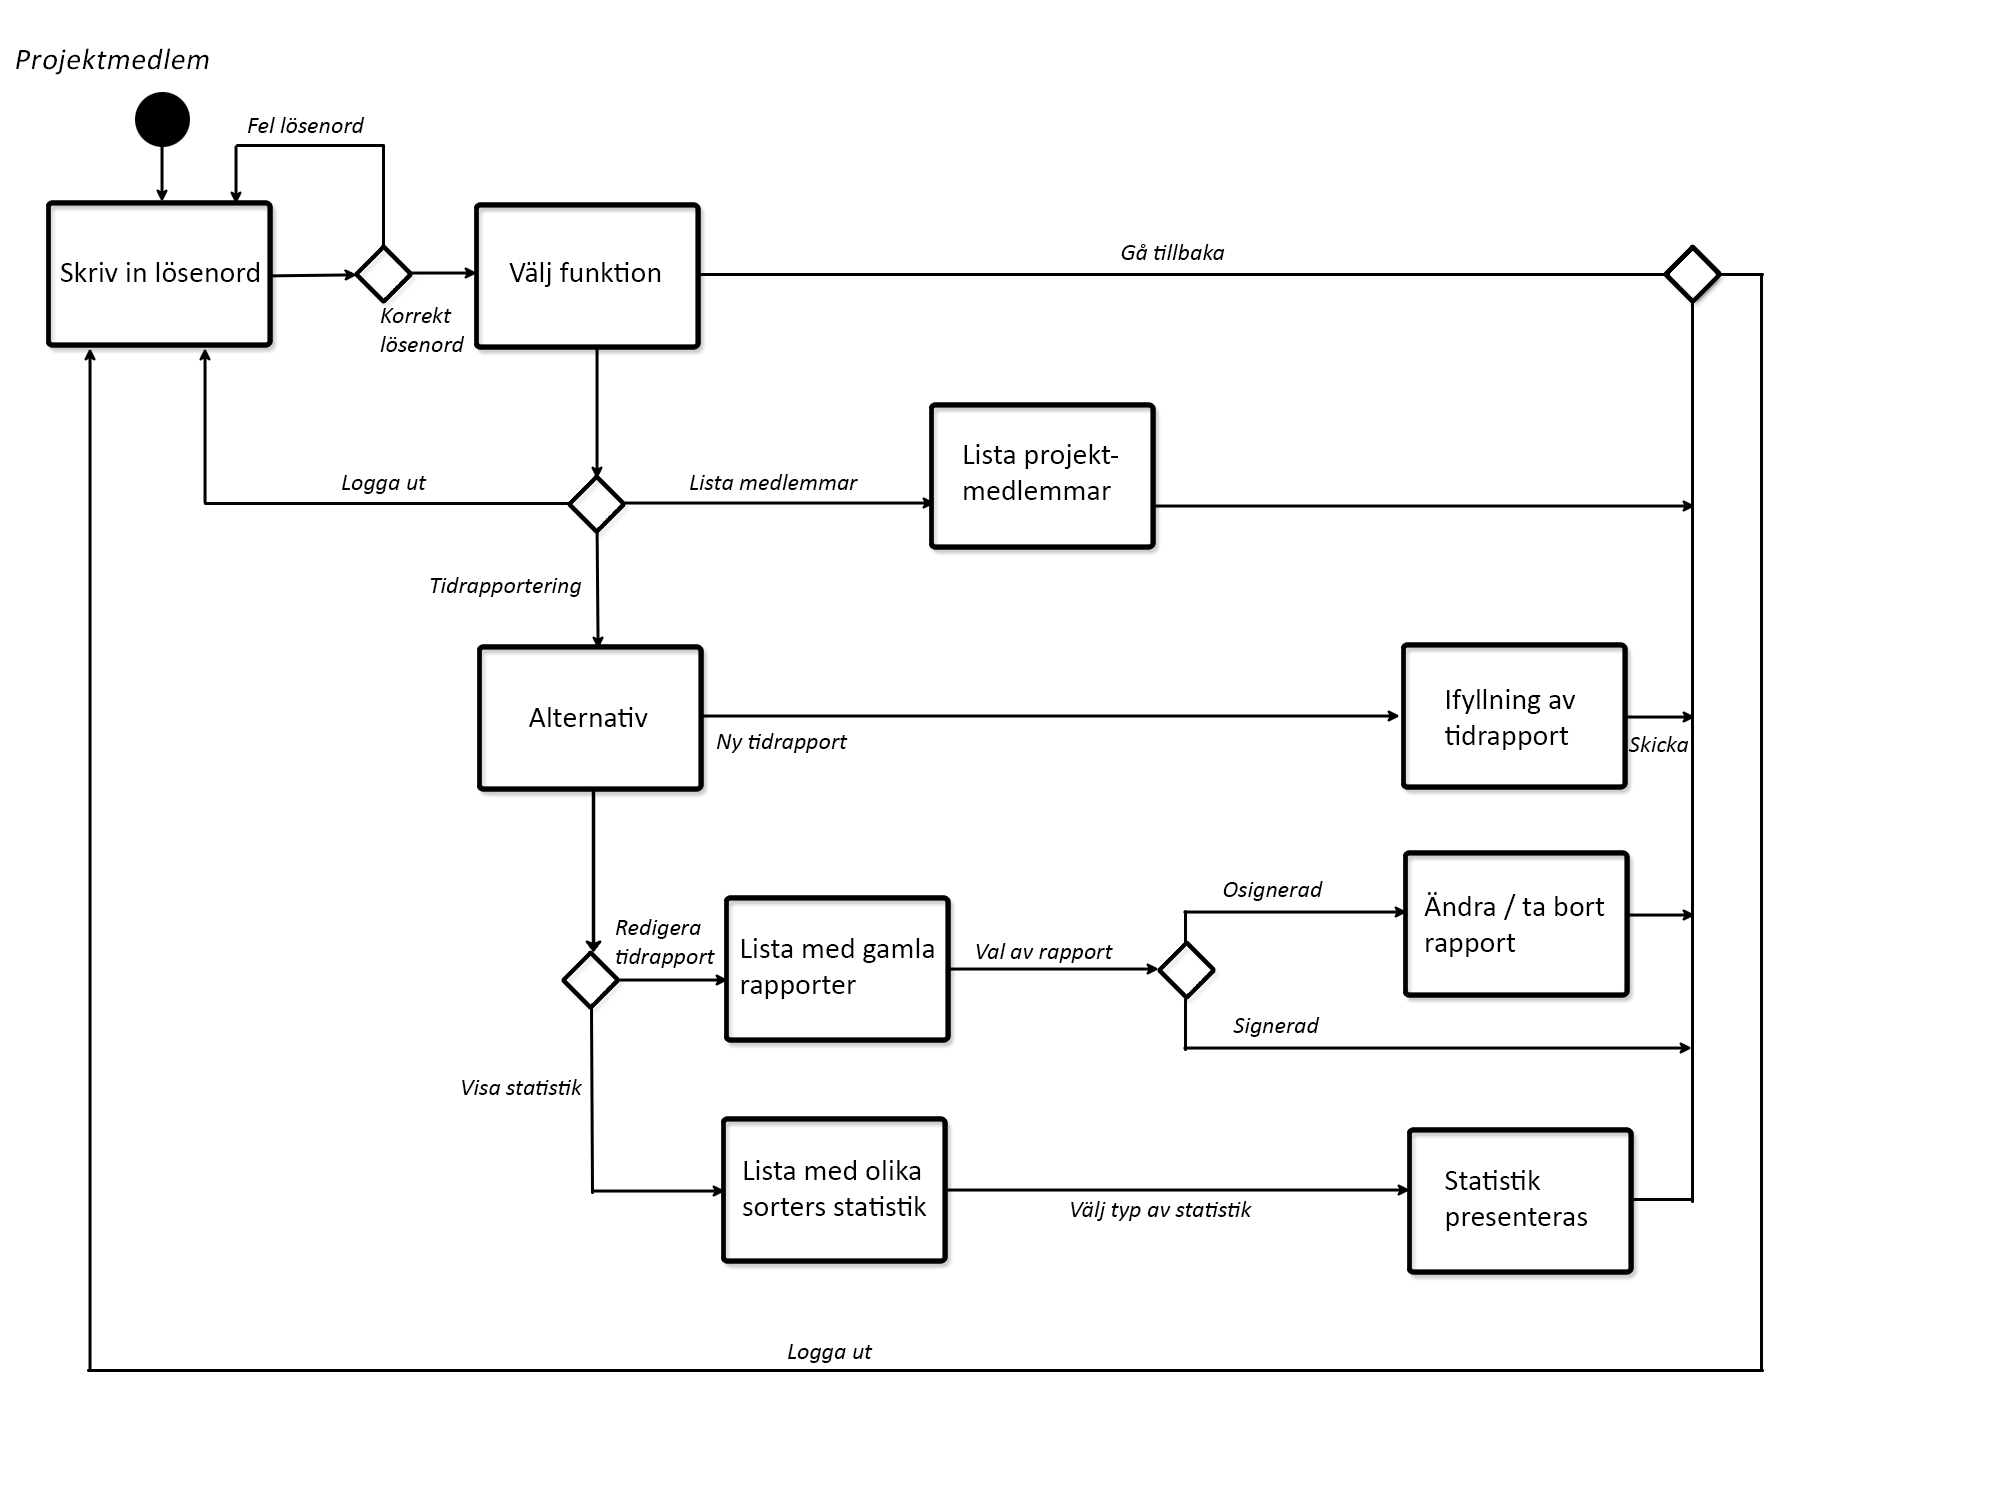
\includegraphics[width=1.1\textwidth,height=0.7\textheight]{flow_time_proj_mem}
\caption{Diagram som visar användarfall för en projektmedlem.}
\label{fig:vertical_offset}
\end{figure}


\item
\textbf{Systemet stödjer stegen i figur 1}

\emph{Starttillstånd:} Projektmedlem A är inte inloggad. Signerad tidrapport y finns i systemet. \\
\emph{Sluttillstånd:} Projektmedlem A är inte inloggad. Osignerad tidrapport x och signerad tidrapport y finns i systemet.\\

\begin{enumerate}

\item A skriver in URL för inloggningssidan.
\item A loggar in, fel lösenord rätt användarnamn. Misslyckas, sidan laddas om.
\item A skriver in rätt lösenord och rätt användarnamn, lyckas, huvudsidan visas.
\item Kontrollera att A kan se projektmedlemsfunktionaliteter på funktionalitetssidan I.\\
\item A väljer ``Lista medlemmar''.
\item Kontrollera att alla projektmedlemmar i As grupp listas.
\item A går tillbaka till I.
\item A väljer ``Tidrapportering''.
\item A väljer ``Ny tidrapport''
\item Fyller i tidrapport, 50 i godtycklig ruta, trycker på ``Skicka'', lyckas. Tidrapport x skapad.
\item A går tillbaka till I.
\item A väljer "Redigera tidrapport".
\item Kontrollera att gamla tidrapporter listas.
\item Väljer tidrapport y, kan inte redigera.
\item A går tillbaka till ``Redigera tidrapport''.
\item A väljer tidrapport x.
\item A ändrar/tar bort rapporten.
\item A väljer ``Visa statistik''.
\item Kontrollera att olika sorters statistik listas (statistik per användare, per roll etc.).\\
\item A genererar statistik per roll, alla veckor.
\item A loggar ut.
\item Kontrollera att A är utloggad.

\end {enumerate}



\end{ST}

\subsubsection{Projektledare}

\begin{figure}
\centering
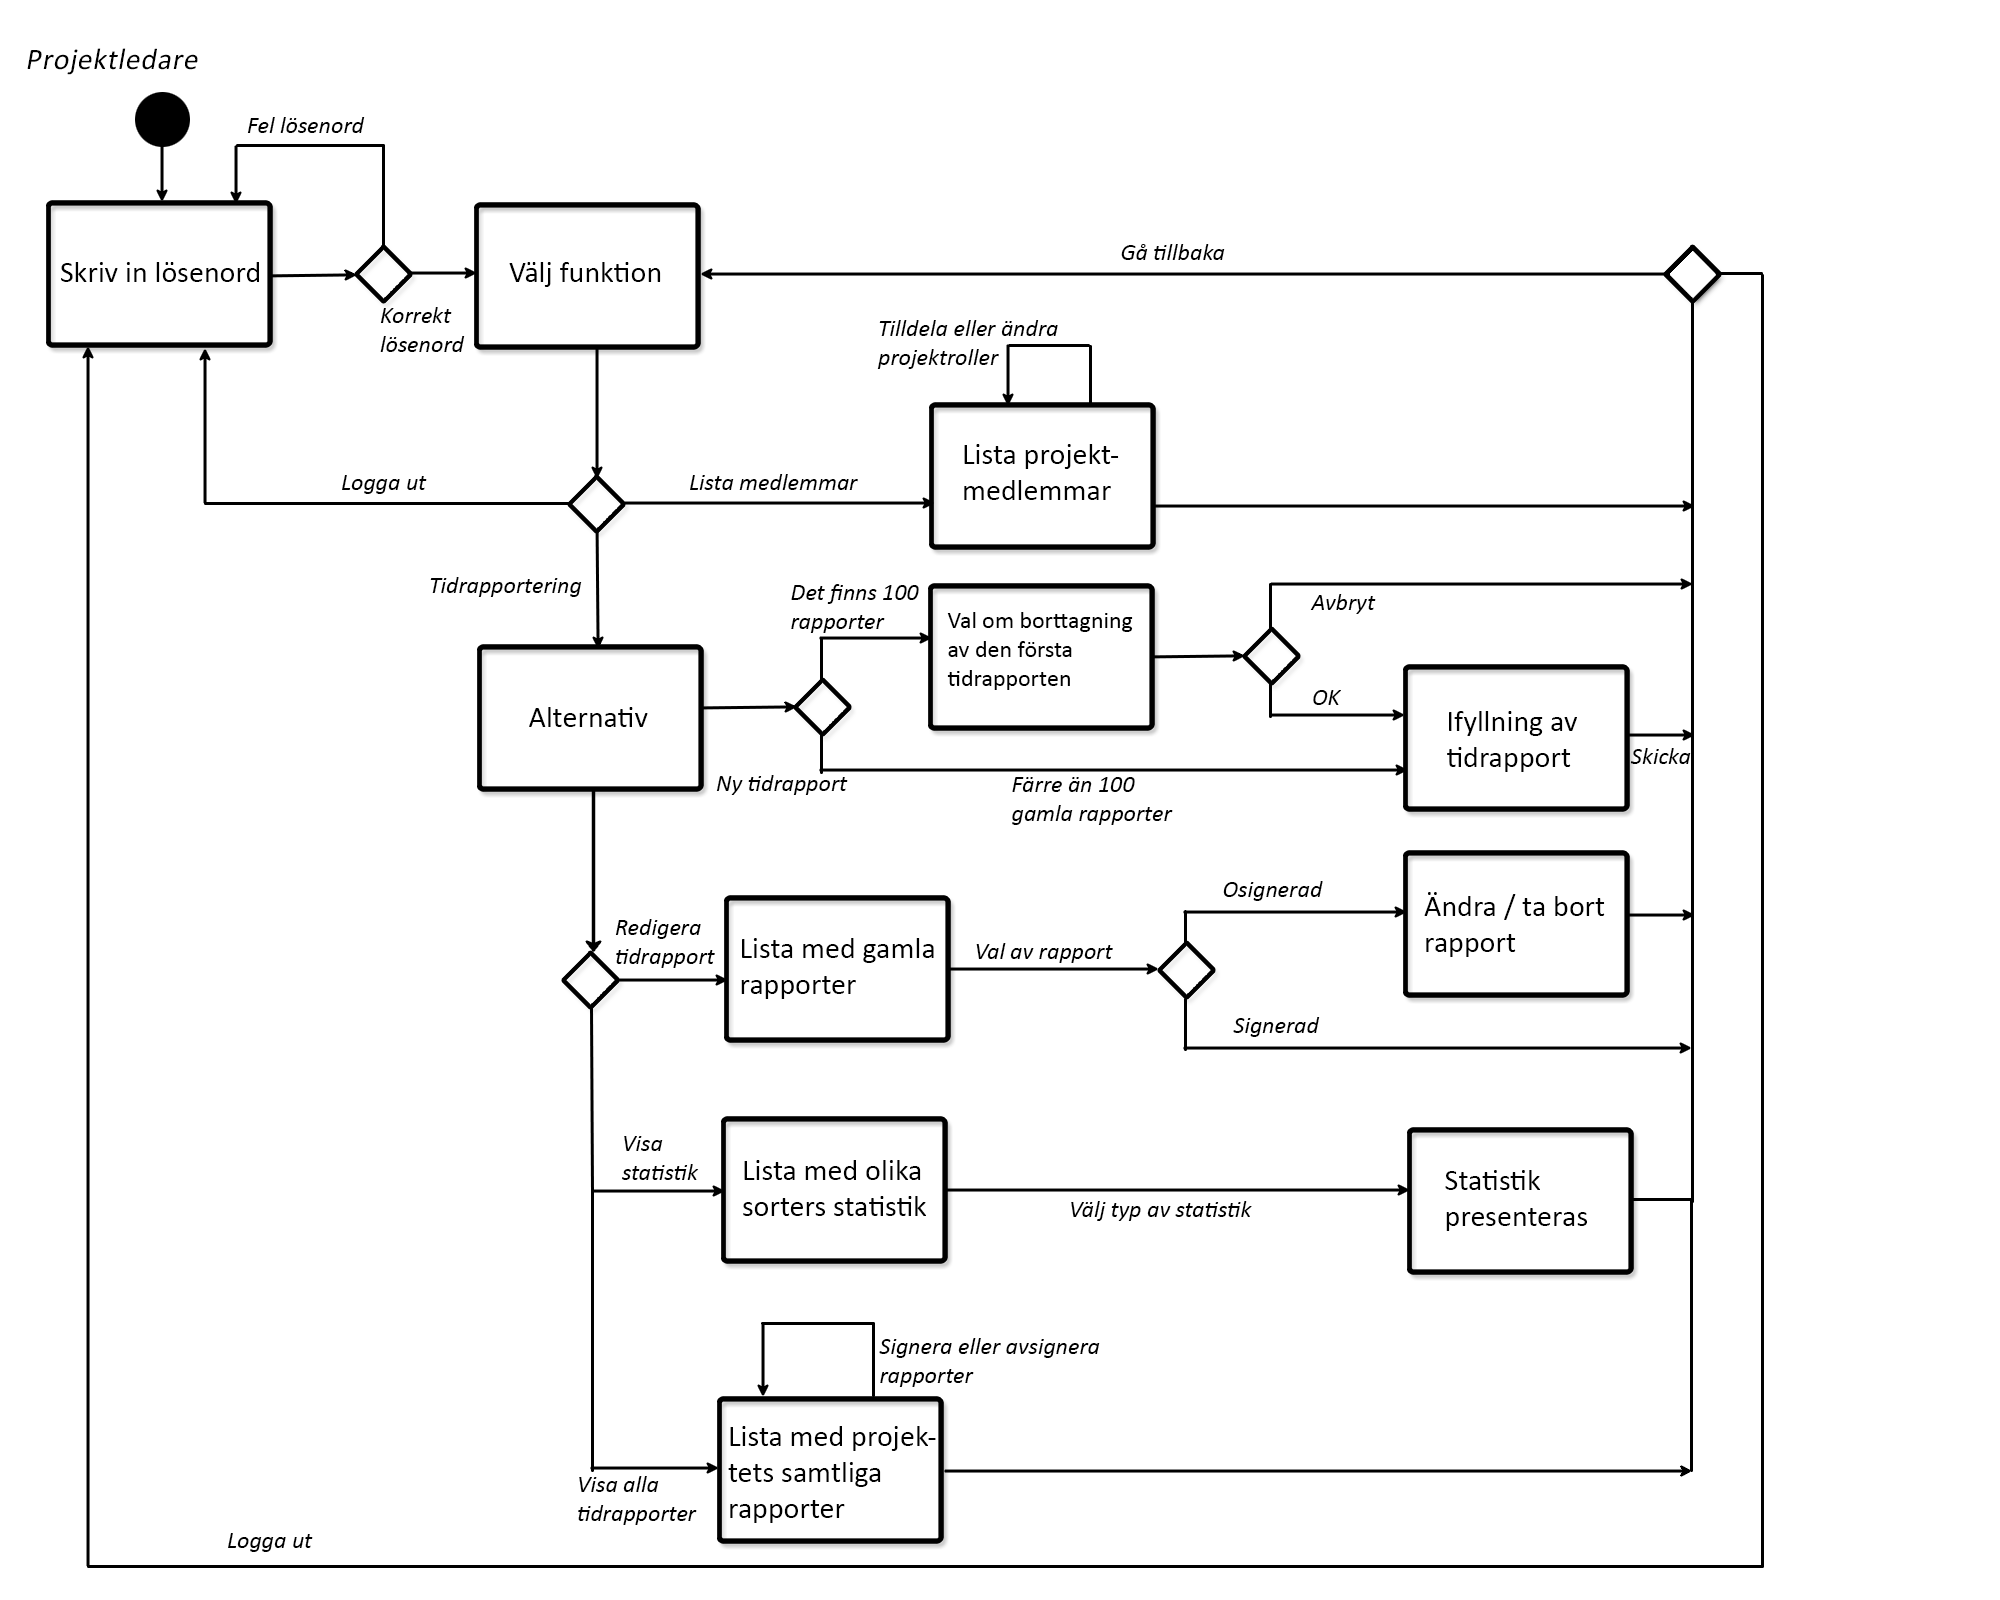
\includegraphics[width=1.1\textwidth,height=0.7\textheight]{flow_time_proj_leader}
\caption{Diagram som visar användarfall för en projektledare.}
\label{fig:vertical_offset}
\end{figure}


%MAX 100 RAPPORTER KRAV INTE MED
\begin{ST}
\item 
\textbf{Systemet stödjer stegen i figur 2}\\
\emph{Starttillstånd:} Projektledare A inte inloggad. Projektmedlem B har rollen t1, en osignerad tidrapport x.\\
\emph{Sluttillstånd:} Projektledare A inte inloggad. Projektmedlem B har rollen t2, en signerad tidrapport x.\\

\begin{enumerate}

\item A skriver in URL till inloggninssidan.
\item A skriver in fel lösenord, rätt användarnamn. Misslyckas, sidan laddas om.
\item A skriver in rätt lösenord och rätt användarnamn. Lyckas logga in.
\item Kontrollera att A har tillgång till projektledarfuntionaliteter.
\item A väljer ``Lista medlemmar''.
\item Kontrollera att A ser alla medlemmar och dess roller.
\item A byter roll på medlem B till t2.
\item A klickar på menyn.
\item A väljer ``Tidrapportering''.
\item A väljer ``Ny tidrapport''.
\item A fyller in ny tidrapport och trycker på ``Skicka''.
\item Kontrollera att tidrapport är skapad.
\item A skriver in URL för ``Tidrapportering''.
\item A trycker ``Redigera tidrapport''.
\item Kontrollera att en lista med tidrapporter kan ses.
\item A försöker redigera/ta bort sin signerade rapport, går inte.
\item A ändrar/tar bort sin osignerade rapport.
\item A skriver URL ``Tidrapportering''.
\item A väljer ``Visa statistik''.
\item Kontrollera att A kan se en lista med statistik (per användare, per roll etc.)
\item A väljer statistik per användare för alla veckor.
\item A trycker ``Generera''.
\item Kontrollera att A kan se statistiken.
\item A skriver URL ``Tidrapportering''.
\item A väljer ``Visa alla tidrapporter''.
\item A väljer projektmedlem B, sätter tidrapport x till godkänd.
\item A loggar ut.
\item Kontrollera att A är utloggad.



\end{enumerate}

\end{ST}
%++++++++++++++++++++++++++%
%SLUT på ST:tidrapportering%
%++++++++++++++++++++++++++%




%+++++++++++++++++++++++++++%
%BÖRJAN på ST:Administration%
%+++++++++++++++++++++++++++%
\subsection{Administration}

\subsubsection{Projektledare}
\begin{ST}

\item
\textbf{Genomför scenario 6.4.1 i SRS som projektledare}

\emph{Starttillstånd:} Projektledare PL inloggad.

\emph{Sluttillstånd:} Projekledare PL inloggad.

\begin{enumerate}
\item
PL väljer "Generera statistik" i menyn
\item
PL väljer [typ av statistik]
\item 
PL väljer [typ av rapport]
\item
Kontrollera att rapport av typ [typ av rapport] visas.
\item
Kontrollera att statistik av typ [typ av statistik] visas.
\end{enumerate}

\item
\textbf{Genomför scenario 6.4.2 i SRS som projektledare}

\emph{Starttillstånd:} Projektledare PL inloggad. En icke godkänd tidsrapport finns i systemet.

\emph{Sluttillstånd:} Projekledare PL inloggad. En godkänd tidsrapport finns i systemet.

\begin{enumerate}

\item
PL väljer att lista tidrapporter
\item
PL väljer en icke godkänd tidrapport ur listan
\item
Kontrollera att PL ser rapporten
\item
PL godkänner rapporten
\item
Kontrollera att dialogruta visades
\item
Kontrollera att rapporten är godkänd

\end{enumerate}

\item
\textbf{Genomför scenario 6.4.3 i SRS som projektledare}

\item
\textbf{Genomför scenario 6.4.4 i SRS som projektledare}

\emph{Starttillstånd:} Projektledare L som är projektledare för grupp G är inloggad och befinner sig på sidan ``Visa statistik''. Det finns tre projektmedlemmar i G utöver L i systemet, M1, M2 och M3. M1 heter ``axelg'', M2 heter ``axelu'', M3 heter ``johan''. De har två tidsrapporteringar var för vecka 1 och 2. M1 har en tidrapport T1a som innehåller 10 minuter registrerat på möte vecka 1 och en tidsrapport T1b som innehåller 15 minuter registrerat på möte vecka 2. M2 har en tidrapport T2a som innehåller 20 minuter registrerat på möte vecka 1 och en tidsrapport T2b som innehåller 25 minuter registrerat på möte vecka 2. M3 har en tidrapport T3a som innehåller 30 minuter registrerat på möte vecka 1 och en tidsrapport T3b som innehåller 35 minuter registrerat på möte vecka 2. Alla tidrapporter för vecka 1 är signerade, alla tidrapporter för vecka 2 är osignerade.

\emph{Sluttillstånd:} Projektledare L som är projektledare för grupp G är inloggad och befinner sig på sidan ``Visa statistik''. Det finns tre projektmedlemmar i G utöver L i systemet, M1, M2 och M3. M1 heter ``axelg'', M2 heter ``axelu'', M3 heter ``johan''. De har två tidsrapporteringar var för vecka 1 och 2. M1 har en tidrapport T1a som innehåller 10 minuter registrerat på möte vecka 1 och en tidsrapport T1b som innehåller 15 minuter registrerat på möte vecka 2. M2 har en tidrapport T2a som innehåller 20 minuter registrerat på möte vecka 1 och en tidsrapport T2b som innehåller 25 minuter registrerat på möte vecka 2. M3 har en tidrapport T3a som innehåller 30 minuter registrerat på möte vecka 1 och en tidsrapport T3b som innehåller 35 minuter registrerat på möte vecka 2. Alla tidrapporter för vecka 1 är signerade, alla tidrapporter för vecka 2 är osignerade.

\begin{enumerate}
\item Tryck på ``Sortera alla tidrapporter efter namn, stigande ordning''.
\item Kontrollera att det är sorterat på ordningen M1, M2 sen M3.
\item Tryck på ``Sortera alla tidrapporter efter vecka, stigande ordning''.
\item Kontrollera att det är sorterat på ordningen vecka 1 sen vecka 2.
\item Tryck på ``Sortera alla tidrapporter efter om rapporten är godkänd eller ej, stigande ordning''.
\item Kontrollera att det är sorterat på ordningen osignerat sen signerat.
\item Tryck på ``Sortera alla tidrapporter efter namn, fallande ordning''.
\item Kontrollera att det är sorterat på ordningen M3, M2 sen M1.
\item Tryck på ``Sortera alla tidrapporter efter vecka, fallande ordning''.
\item Kontrollera att det är sorterat på ordningen vecka 2 sen vecka 1.
\item Tryck på ``Sortera alla tidrapporter efter om rapporten är godkänd eller ej, fallande ordning''.
\item Kontrollera att det är sorterat på ordningen signerat sen osignerat.
\end{enumerate}

\end{ST}

\subsubsection{Administratör}

\begin{ST}

\item
\textbf{Genomför scenario 6.4.1 i SRS som administratör}

\emph{Starttillstånd:} Administratör A inloggad.

\emph{Sluttillstånd:} Administratör A inloggad.

\begin{enumerate}
\item
A väljer "Generera statistik" i menyn
\item
A väljer [typ av statistik]
\item 
A väljer [typ av rapport]
\item
Kontrollera att rapport av typ [typ av rapport] visas.
\item
Kontrollera att statistik av typ [typ av statistik] visas.
\end{enumerate}

\item
\textbf{Genomför scenario 6.4.2 i SRS som administratör}

\emph{Starttillstånd:} Administratör A inloggad. En icke godkänd tidsrapport finns i systemet.

\emph{Sluttillstånd:} Administratör A inloggad. En godkänd tidsrapport finns i systemet.

\begin{enumerate}

\item
A väljer att lista tidrapporter
\item
A väljer en icke godkänd tidrapport ur listan
\item
Kontrollera att A ser rapporten
\item
A godkänner rapporten
\item
Kontrollera att dialogruta visades
\item
Kontrollera att rapporten är godkänd

\end{enumerate}

\item
\textbf{Genomför scenario 6.4.3 i SRS som administratör}

\emph{Starttillstånd:} Projektledare A inloggad. Inne på sidan för tidrapportering. Rapport x godkänd.\\
\emph{Sluttillstånd:} Projektledare A inloggad. Inne på sidan för tidrapportering. Rapport x inte godkänd.\\


\begin{enumerate}
\item A listar alla tidrapporter
\item A väljer rapport x, trycker på "Ej godkänd"
\item Kontrollera att en dialogruta kommer fram som bekräftar att x inte är godkänd.
\item Kontrollera att x inte är godkänd.
\item Kontrollera att A dirigeras tillbaka till sidan över alla tidrapporter.
\end{enumerate}

\item
\textbf{Genomför scenario 6.4.4 i SRS som administratör}

\emph{Starttillstånd:} Administratören A är inloggad och befinner sig på sidan ``Visa statistik''. Det finns tre projektmedlemmar i projektgruppen G i systemet, M1, M2 och M3. M1 heter ``axelg'', M2 heter ``axelu'', M3 heter ``johan''. De har två tidsrapporteringar var för vecka 1 och 2. M1 har en tidrapport T1a som innehåller 10 minuter registrerat på möte vecka 1 och en tidsrapport T1b som innehåller 15 minuter registrerat på möte vecka 2. M2 har en tidrapport T2a som innehåller 20 minuter registrerat på möte vecka 1 och en tidsrapport T2b som innehåller 25 minuter registrerat på möte vecka 2. M3 har en tidrapport T3a som innehåller 30 minuter registrerat på möte vecka 1 och en tidsrapport T3b som innehåller 35 minuter registrerat på möte vecka 2. Alla tidrapporter för vecka 1 är signerade, alla tidrapporter för vecka 2 är osignerade.

\emph{Sluttillstånd:} Administratören A är inloggad och befinner sig på sidan ``Visa statistik''. Det finns tre projektmedlemmar i projektgruppen G i systemet, M1, M2 och M3. M1 heter ``axelg'', M2 heter ``axelu'', M3 heter ``johan''. De har två tidsrapporteringar var för vecka 1 och 2. M1 har en tidrapport T1a som innehåller 10 minuter registrerat på möte vecka 1 och en tidsrapport T1b som innehåller 15 minuter registrerat på möte vecka 2. M2 har en tidrapport T2a som innehåller 20 minuter registrerat på möte vecka 1 och en tidsrapport T2b som innehåller 25 minuter registrerat på möte vecka 2. M3 har en tidrapport T3a som innehåller 30 minuter registrerat på möte vecka 1 och en tidsrapport T3b som innehåller 35 minuter registrerat på möte vecka 2. Alla tidrapporter för vecka 1 är signerade, alla tidrapporter för vecka 2 är osignerade.

\begin{enumerate}
\item Tryck på ``Sortera alla tidrapporter efter namn, stigande ordning''.
\item Kontrollera att det är sorterat på ordningen M1, M2 sen M3.
\item Tryck på ``Sortera alla tidrapporter efter vecka, stigande ordning''.
\item Kontrollera att det är sorterat på ordningen vecka 1 sen vecka 2.
\item Tryck på ``Sortera alla tidrapporter efter om rapporten är godkänd eller ej, stigande ordning''.
\item Kontrollera att det är sorterat på ordningen osignerat sen signerat.
\item Tryck på ``Sortera alla tidrapporter efter namn, fallande ordning''.
\item Kontrollera att det är sorterat på ordningen M3, M2 sen M1.
\item Tryck på ``Sortera alla tidrapporter efter vecka, fallande ordning''.
\item Kontrollera att det är sorterat på ordningen vecka 2 sen vecka 1.
\item Tryck på ``Sortera alla tidrapporter efter om rapporten är godkänd eller ej, fallande ordning''.
\item Kontrollera att det är sorterat på ordningen signerat sen osignerat.
\end{enumerate}

\item \textbf{Administratören har tillgång administratörsfunktionaliteter} 

\emph{Starttillstånd:} Administratör Ad är inte inloggad.

\emph{Sluttillstånd:} Administratör Ad är inte inloggad.

\begin{enumerate}
\item Ad skriver URL till inloggningssidan.
\item Ad skriver felaktigt lösenord, sidan laddas om.
\item Ad skriver rätt lösenord, inloggad.
\item Ad väljer administrationsvyn.
\item Ad väljer funk. lista användare.
\item Kontrollera att Ad kan se alla användare med lösenord.
\item Ad lägger till användare, rätt input, lyckas.
\item Ad försöker lägga till användare, fel input, misslyckas.
\item Ad tar bort användare, lyckas.
\item Ad väljer administrationsvyn.
\item Ad väljer funk. Projektgrupper.
\item Ad lägger till användare i godtycklig projektgrupp, lyckas.
\item Ad tar bort användare från projektgrupp, lyckas.
\item Ad försöker ta bort projektgrupp, finns projektmedlemmar i, misslyckas.
\item Ad tar bort projektgrupp, tom projektgrupp, lyckas.
\item Ad skapar projektgrupp.
\item Ad väljer tidrapportmall.
\item Ad väljer användare till projektgruppen från en lista.
\item Ad väljer projektledare, trycker på "Skapa".
\item Kontrollera att Ad skickas tillbaka till administrationsvyn.
\item Steg 11-20 upprepas, men i steg 17 skapar Ad en ny tidrapportmall.
\item Ad väljer funk. Redigera projektmedlemmar.
\item Kontrollera att samtliga projektmedlemmar listas.
\item Ad utser andra projektledare, lyckas.
\item Ad tilldelar roller, lyckas.
\item Ad byter grupp på användare, lyckas.
\item Ad väljer väljer administrationsvyn.
\item Ad väljer funk. Ta bort tidrapportmall.
\item Kontrollera att tidrapportmallarna listas.
\item Ad försöker ta bort tidrapportmall som används, misslyckas.
\item Ad tar bort tidrapportmall som inte används, lyckas.
\item Ad väljer administrationsvyn.
\item Ad trycker på "Logga ut".
\item Kontrollera att Ad är utloggad.
\end{enumerate}

\end{ST}



%+++++++++++++++++++++++++++%
%SLUTET på ST:Administration%
%+++++++++++++++++++++++++++%




%+++++++++++++++++++++++++++%
%BÖRJAN på ST:Kvalitetstest+%
%+++++++++++++++++++++++++++%
\subsection{Kvalitetskrav}

\subsubsection{Prestanda}

\begin{ST}
\item
\textbf{Försök logga in med fler än 50 användare samtidigt.}

\emph{Starttillstånd:} Användare user1-user51 finns registrerade med lösenord pass. Inga användare inloggade.

\emph{Sluttillstånd:} Användare user1-user50 är inloggade. User51 är inte inloggad

\begin{enumerate}

\item
Försök logga in användare user1-user51.
\item
Kontrollera att user1-user50 är inloggade.
\item
Kontrollera att user51 inte är inloggad.
\end{enumerate}

\item
\textbf{Logga in med 50 användare}

\emph{Starttillstånd:} Användare user1-user50 finns registrerade med lösenord pass. Inga användare inloggade.

\emph{Sluttillstånd:} Användare user1-user50 är inloggade.

\begin{enumerate}

\item
Försök logga in användare user1-user50.
\item
Kontrollera att user1-user50 är inloggade.
\end{enumerate}


\item
\textbf{Svaret på en godtycklig förfrågan från en dator i E-huset kommer i 95\% av fallen tillbaka
inom en sekund.}

\emph{Starttillstånd:} Administratör inloggad på dator i E-huset.

\emph{Sluttillstånd:} Administratör inloggad på dator i E-huset.

\begin{enumerate}

\item Administratören försöker generera statistik 40 gånger. Tiden det tar innan servern svarar mäts varje gång.

\item Den uppmätta tiden utvärderas och bör inte vara högre än en (1) sekund fler än två (2) gånger.


\end{enumerate}

\end{ST}

%+++++++++++++++++++++++++++%
%SLUTET på ST:Kvalitetstest+%
%+++++++++++++++++++++++++++%
%\end{ST}
\subsection{Regressionstest}

Alla test ska köras två gånger i veckan.

När något ändras ska helst alla tester köras igen. Om så inte är möjligt ska åtminstone de
generella kraven och de tester i det område som förändringen påverkade köras.
Om något ändras inom dessa områden måste följande testfall regressionstestas. Vid varje
ändring ska de test rörande de generella kraven också testas.
Områden innefattar:

\begin{itemize}

\item
Generella krav

\item
Autentisering

\item
Tidrapportering

\item
Administration

\end{itemize}


\end{document}
